%% Recomendaciones seguidas: http://www.fi.upm.es/?pagina=1475
%% - Paginas: DIN A4, a doble cara
%% - Portada: en breve se publicara un ejemplo
%% - Letra: Times Roman 12 puntos o equivalente en negro
%% - Márgenes: superior e inferior 3,5 cm, izquierdo y derecho 3 cm.
%% - Superficie del texto: 22,5 cm. de alto (aproximadamente 40
%%   líneas) y 15 cm. de ancho
%% - Cabecera y pies: fuera de la superficie del texto
%% - Secciones y subsecciones: reseñadas con numeración decimal a
%%   continuación del número del capítulo. Ej.: subsecciones 2.3.1.
%% - Títulos de capítulos: en letra mayúscula
%% - Números de página: siempre centrado en margen inferior, página 1
%%   comienza en capítulo 1, todas la secciones precedentes al
%%   capítulo 1 en número romano (en minúscula)
%% - Bibliografía: según las recomendaciones de la IEEE
%%   (http://www.fi.upm.es/docs/estudios/grado/1475_ieeecitationref.pdf)

\documentclass[twoside,12pt]{book}
\usepackage[
a4paper,
bindingoffset=10mm,
hmargin=30mm,
vmargin=35mm,
textwidth=150mm,
textheight=225mm]{geometry}
\linespread{1.1} % Para forzar unas 40 líneas
\setlength{\parskip}{1.5ex}

%%%%%%%%%%%%%%%%%%%%%%%%%%%%%%%%%%%%%%%%%%%%%%%%%%%%%%%%%%%%%%%%%%%%%%%%
% Codificación de caracteres
\usepackage[utf8]{inputenc}

%%%%%%%%%%%%%%%%%%%%%%%%%%%%%%%%%%%%%%%%%%%%%%%%%%%%%%%%%%%%%%%%%%%%%%%%
% Selección del lenguaje
\usepackage[spanish,english]{babel}

%%%%%%%%%%%%%%%%%%%%%%%%%%%%%%%%%%%%%%%%%%%%%%%%%%%%%%%%%%%%%%%%%%%%%%%%
%% Cabeceras
\usepackage{fancyhdr}

%%%%%%%%%%%%%%%%%%%%%%%%%%%%%%%%%%%%%%%%%%%%%%%%%%%%%%%%%%%%%%%%%%%%%%%%
%% Gráficos
\usepackage[final]{graphicx}

%%%%%%%%%%%%%%%%%%%%%%%%%%%%%%%%%%%%%%%%%%%%%%%%%%%%%%%%%%%%%%%%%%%%%%%%
\usepackage{ifdraft}

%%%%%%%%%%%%%%%%%%%%%%%%%%%%%%%%%%%%%%%%%%%%%%%%%%%%%%%%%%%%%%%%%%%%%%%%
%% Tipos de letra
\usepackage{kmath,kerkis}
\usepackage[scaled=0.83]{helvet} %% Helvetica queda demasiado grande
\usepackage[scaled=0.75]{beramono}
\usepackage[T1]{fontenc}

\newcommand{\dedicafont}{\usefont{T1}{phv}{m}{n}\fontsize{14}{17.5}\selectfont}
\newcommand*{\copyrightfont}{\usefont{T1}{phv}{m}{n}\fontsize{6}{7.5}\selectfont}
\newcommand{\sectionalfont}{\usefont{T1}{phv}{b}{n}}
% {64}{80} {56}{70} {48}{60} {32}{40} {24}{30} {18}{22.5} {16}{20} {14}{17.5} {12}{15}
\newcommand{\partnumberfont}{\sectionalfont\fontsize{64}{80}\selectfont}
\newcommand{\parttitlefont}{\sectionalfont\fontsize{48}{60}\selectfont}
\newcommand{\chapternumberfont}{\sectionalfont\fontsize{64}{80}\selectfont}
\newcommand{\chaptertitlefont}{\sectionalfont\fontsize{32}{40}\selectfont}
\newcommand{\sectiontitlefont}{\sectionalfont\fontsize{18}{22.5}\selectfont}
\newcommand{\subsectiontitlefont}{\sectionalfont\fontsize{16}{20}\selectfont}
\newcommand{\subsubsectiontitlefont}{\sectionalfont\fontsize{14}{17.5}\selectfont}
\newcommand{\headertitlefont}{\sectionalfont\fontsize{12}{15}\selectfont}

%%%%%%%%%%%%%%%%%%%%%%%%%%%%%%%%%%%%%%%%%%%%%%%%%%%%%%%%%%%%%%%%%%%%%%%%
%% Tipos de letra en cabeceras de secciones
\usepackage{titlesec}

\titleformat{\part} % command
[display] % shape
{} % format
{\partnumberfont\flushright Part\quad\thepart} % label
{0pt} % sep
{\parttitlefont\flushright} % before
[] % after

\titleformat{\chapter} % command
[display] % shape
{} % format
{\chapternumberfont\flushright\thechapter} % label
{0pt} % sep
{\chaptertitlefont\flushright} % before
[] % after

\titleformat*{\section}{\sectiontitlefont}

\titleformat*{\subsection}{\subsectiontitlefont}

\titleformat*{\subsubsection}{\subsubsectiontitlefont}

%%%%%%%%%%%%%%%%%%%%%%%%%%%%%%%%%%%%%%%%%%%%%%%%%%%%%%%%%%%%%%%%%%%%%%%%
%% Macros para este TFC
\newcommand{\titulo}{Adaptación servicios web BetFair al sistema móvil iOS}
\newcommand{\autor}{Francisco Miguel Merchan Casado}
\newcommand{\tutor}{Ángel Herranz Nieva}
\newcommand{\fecha}{Julio 2012}

% Cleardoublepage
\makeatletter
\def\cleardoublepage{\clearpage\if@twoside \ifodd\c@page\else
\hbox{}
\vspace*{\fill}
\begin{center}
% This page intentionally contains only this sentence.
\end{center}
\vspace{\fill}
\thispagestyle{empty}
\newpage
\if@twocolumn\hbox{}\newpage\fi\fi\fi}
\makeatother

\usepackage{url}

\usepackage{hyperref}

\usepackage{eurosym}

\usepackage{dcolumn} % Formato Tabla
\usepackage{colortbl} 
\usepackage{longtable}
\usepackage{tabularx}
\usepackage{supertabular}

\usepackage{color}	% Formato codigo
\definecolor{gray97}{gray}{.97}
\definecolor{gray75}{gray}{.75}
\definecolor{gray45}{gray}{.45}
 
\usepackage{listings}
\lstset{
     basicstyle=\ttfamily,
     % showstringspaces = false,
     commentstyle=\color{gray45},
     keywordstyle=\color{blue},
     %
     frame=single,
     aboveskip=0.5cm,
     framextopmargin=3pt,
     framexbottommargin=3pt,
     framexleftmargin=0.4cm,
     framesep=0pt,
     rulesep=.4pt,
     backgroundcolor=\color{gray97},
     rulesepcolor=\color{black},
     %
     numbers=left,
     numbersep=15pt,
     numberstyle=\tiny,
     numberfirstline = false,
     breaklines=true,
   }

%% Fixmes
%% macros: \fixme -critical-, \fxerror -noncritical-, \fxwarning, \fxnote
%% env: afixme, anfxerror, anfxwarning, anfxnote
% % \usepackage[marginclue,inline]{fixme}
\usepackage[inline,nomargin,draft]{fixme}
%% \usepackage[marginclue,footnote]{fixme}
\usepackage{framed}
%%\renewcommand{\FXInline}[2]{\noindent{\color{red}#1: \emph{\small #2}}}
%%\renewcommand{\FXMarginClue}[1]{\marginpar{\footnotesize\raggedleft\textbf{\color{red}#1~!}}}
%%\renewcommand{\FXEnvBegin}{\begin{framed}\begin{small}\color{red}}
%%\renewcommand{\FXEnvEnd}{\end{small}\end{framed}}
\usepackage{float}
%%%%%%%%%%%%%%%%%%%%%%%%%%%%%%%%%%%%%%%%%%%%%%%%%%%%%%%%%%%%%%%%%%%%%%%%
%%%%%%%%%%%%%%%%%%%%%%%%%%%%%%%%%%%%%%%%%%%%%%%%%%%%%%%%%%%%%%%%%%%%%%%%
%% Comienza en libro
\begin{document}

%%%%%%%%%%%%%%%%%%%%%%%%%%%%%%%%%%%%%%%%%%%%%%%%%%%%%%%%%%%%%%%%%%%%%%
%% SELECCIÓN DEL IDIOMA
%% (NO TOCAR: SÓLO SE ADMITE ESPAÑOL)
%% (VER summary.tex para activar otro idioma, ej. inglés)
\selectlanguage{spanish}

%%%%%%%%%%%%%%%%%%%%%%%%%%%%%%%%%%%%%%%%%%%%%%%%%%%%%%%%%%%%%%%%%%%%%%%%
%%%%%%%%%%%%%%%%%%%%%%%%%%%%%%%%%%%%%%%%%%%%%%%%%%%%%%%%%%%%%%%%%%%%%%%%
%% Portada, dedicatoria, índices, agradecimientos y resúmenes
\pagestyle{empty}

\thispagestyle{empty}

\begin{tabular}{cc}
  \begin{minipage}{2cm}
%    \hspace*{-2em}
    
\includegraphics[width=2cm]{logos/logofiBN}
  \end{minipage}
  &
  \begin{minipage}{0.75\textwidth}
    \begin{large}
      UNIVERSIDAD POLITÉCNICA DE MADRID\\[1ex]
      FACULTAD DE INFORMÁTICA
    \end{large}
  \end{minipage}
\end{tabular}

\vfill

\begin{center}
  \begin{LARGE}
    TRABAJO FIN DE CARRERA
  \end{LARGE}
\end{center}

\vfill

\begin{center}
  \begin{LARGE}
    \titulo
  \end{LARGE}
\end{center}

\vfill

\begin{center}
  \begin{LARGE}
    AUTOR: \textrm{\autor}\\[1ex]
    TUTOR: \textrm{\tutor}\\[2ex]
    \fecha
  \end{LARGE}
\end{center}

%%% Local Variables: 
%%% mode: latex
%%% TeX-master: "tfc-betfair-ios"
%%% TeX-PDF-mode: t
%%% ispell-local-dictionary: "castellano"
%%% End: 

\cleardoublepage

\hfill
\begin{textit}
  A mi querido abuelo Santiago.
\end{textit}

%%% Local Variables: 
%%% mode: latex
%%% TeX-master: "tfc-betfair-ios"
%%% TeX-PDF-mode: t
%%% ispell-local-dictionary: "castellano"
%%% End: 

\cleardoublepage

\pagestyle{plain}
\pagenumbering{roman}

%%%%%%%%%%%%%%%%%%%%%%%%%%%%%%%%%%%%%%%%%%%%%%%%%%%%%%%%%%%%%%%%%%%%%%
%% ÍNDICE GENERAL
%% (NO TOCAR)
\tableofcontents
\cleardoublepage

%%%%%%%%%%%%%%%%%%%%%%%%%%%%%%%%%%%%%%%%%%%%%%%%%%%%%%%%%%%%%%%%%%%%%%
%% ÍNDICE DE FIGURAS
%% (COMENTAR SI NO HAY FIGURAS)
\listoffigures
\cleardoublepage

% %%%%%%%%%%%%%%%%%%%%%%%%%%%%%%%%%%%%%%%%%%%%%%%%%%%%%%%%%%%%%%%%%%%%%%
% %% ÍNDICE DE TABLAS
% %% (COMENTAR SI NO HAY TABLAS)
% \listoftables
% \cleardoublepage

%%% Local Variables: 
%%% mode: latex
%%% TeX-master: "tfc-betfair-ios"
%%% TeX-PDF-mode: t
%%% ispell-local-dictionary: "castellano"
%%% End: 

\cleardoublepage

\chapter*{Agradecimientos}

Agradezco a \ldots

%%% Local Variables: 
%%% mode: latex
%%% TeX-master: "tfc-betfair-ios"
%%% TeX-PDF-mode: t
%%% ispell-local-dictionary: "castellano"
%%% End: 

\cleardoublepage

\chapter*{Resumen}
\addcontentsline{toc}{chapter}{Resumen}

En este documento se describe el trabajo de fin de carrera acerca del desarrollo de una aplicación de apuestas para los dispositivos móviles iOS\footnote{iPhone Operating System}. Esta aplicación principalmente contiene las siguientes funcionalidades:
\begin{itemize}
    \item Apostar usando los servicios del portal de apuestas elegido.
    \item Asesoramiento sobre apuestas ya realizadas.
    \item Soporte multi-idioma.
  \end{itemize}
       
      Para ello, principalmente, se han tenido que adaptar los servicios web proporcionados por el portal de apuestas a la plataforma \emph{iOS} haciendo uso de las herramientas de desarrollo de Apple.
       
     En el capítulo \ref{ch:intro} se presentan los conceptos básicos
    de las apuestas deportivas.

%%% Local Variables: 
%%% mode: latex
%%% TeX-master: "tfc-betfair-ios"
%%% TeX-PDF-mode: t
%%% ispell-local-dictionary: "castellano"
%%% End: 

\cleardoublepage

\begin{otherlanguage}{english}

\chapter*{Summary}
\addcontentsline{toc}{chapter}{Summary}

(Summary here)\fxnote{traducir el resumen del español al inglés.}

\end{otherlanguage}

%%% Local Variables: 
%%% mode: latex
%%% TeX-master: "tfc-betfair-ios"
%%% TeX-PDF-mode: t
%%% ispell-local-dictionary: "castellano"
%%% End: 

\cleardoublepage

%%%%%%%%%%%%%%%%%%%%%%%%%%%%%%%%%%%%%%%%%%%%%%%%%%%%%%%%%%%%%%%%%%%%%%%%
%%%%%%%%%%%%%%%%%%%%%%%%%%%%%%%%%%%%%%%%%%%%%%%%%%%%%%%%%%%%%%%%%%%%%%%%
%% Capítulos

%%%%%%%%%%%%%%%%%%%%%%%%%%%%%%%%%%%%%%%%%%%%%%%%%%%%%%%%%%%%%%%%%%%%%%%%
%% Cabeceras
\pagestyle{fancy}
% Remembering the chapter title:
\renewcommand{\chaptermark}[1]{\markboth{\headertitlefont\thechapter\quad#1}{}}
% Remembering section number and title:
\renewcommand{\sectionmark}[1]{\markright{\headertitlefont\thesection\quad#1}}
\fancyhead{} % Clear all header fields
\fancyhead[LE]{\leftmark}
\fancyhead[RO]{\rightmark}
\fancyfoot{} % Clear all footer fields
\fancyfoot[C]{\thepage}
\renewcommand{\headrulewidth}{0pt}
\renewcommand{\footrulewidth}{0pt}
\pagenumbering{arabic}

%%%%%%%%%%%%%%%%%%%%%%%%%%%%%%%%%%%%%%%%%%%%%%%%%%%%%%%%%%%%%%%%%%%%%%
%% CAPÍTULOS:
%%  * PONER CADA CAPÍTULO EN UN FICHERO
%%  * AÑADIR \cleardoublepage DESPUÉS DE CADA input
\chapter{INTRODUCCIÓN}
\label{ch:intro}

En este capítulo, se introduce al lector en el dominio de las apuestas deportivas en Internet y se presenta el terminal elegido como plataforma para la aplicación de apuestas, resultado del presente trabajo de fin de carrera.

\section{Apuestas por Internet}

Actualmente las apuestas tienen gran aceptación comercial en todo el mundo. En España ya existe una tradición de bastantes años por la quiniela y la lotería. En la quiniela, por ejemplo, nunca sabemos por anticipado cuánto cobraremos en caso de acierto ya que depende del número de participantes que hayan acertado el resultado de la jornada de la Liga Profesional de Fútbol. Un acierto de 13 resultados puede convertirse en una gran decepción por el premio conseguido si junto con nosotros han acertado el resultado otras 10000 personas. Sin embargo, si eres el único acertante ya no tienes que repartir el premio. 
 Hace unos pocos años proliferaban las casas de apuestas tradicionales. En estas el apostante cruza su apuesta directamente contra la propia casa. En un típico ejemplo tenemos las clásicas carreras de caballos sobre las que se apuesta sobre un caballo ganador. La casa de apuesta tradicional se limita siempre a cubrir nuestras apuestas asesorados por expertos y siempre con el objetivo de asegurar ganancia sobre el total de las apuestas abierta, por ejemplo, mediante comisiones. 
En los últimos años hemos sido testigos de la llegada de las llamadas casas de intercambio. 
Las casas de intercambio añaden un nuevo concepto en el mundo de las apuestas. Los usuarios realizan las apuestas sobre los eventos y entre ellos mismos se cubren las apuestas, es decir, los apostantes pueden realizar apuestas a favor o en contra de los eventos. 
 En este caso, la casa de apuestas hace de intermediario obteniendo un porcentaje en la ganancia del apostante, una comisión que se calcula sobre la ganancia neta obtenida por el usuario.
 Las ventajas para los clientes de las casas de apuestas de intercambio con respecto a las tradicionales son:
\begin{itemize}
	\item Las comisiones son menores que las correspondientes a una casa de apuestas tradicionales.
	\item Cuanto mayores sean las cantidades apostadas, mayor será la comisión que se lleve la casa de intercambio, es por eso que no suelen existir límites en las cantidades a apostar en contra de las casas de apuestas tradicionales siempre y cuando se cubra una apuesta a favor con otro en contra.
\end{itemize}
Pero como en toda comparación siempre hay desventajas para el cliente: 
\begin{itemize}
	\item Normalmente, debido a las nuevas posibilidades de apuesta de las casas de intercambio se requieren conocimientos avanzados y una mayor experiencia para obtener beneficios en contraposición a la simplicidad que ofrecen las casas de apuestas tradicionales.
	\item En las casas de intercambio son los propios usuarios los que proponen sus apuestas y los mercados tardan más tiempo en abrirse. Se necesita que aparezca un apostante para abrir el mercado. Entendemos por mercado el evento deportivo por el cual podemos apostar a favor o en contra. Por ejemplo, en un partido de tenis apostar por cuál de los dos jugadores va a ganar. En las casas de apuestas tradicionales es la propia casa la que establece las cuotas abriendo los mercados más rápidamente.
\end{itemize}

Debido a la aparición de estas casas de intercambio, aparecen una nueva modalidad para realizar apuestas: el poder realizar apuestas en contra de un evento (\emph{lay}) . Esta es la principal diferencia clara con las casas de apuestas tradicionales donde sólo se pueden realizar apuestas a favor (\emph{back}) de un evento.
 Con esta nueva modalidad para realizar apuestas se facilita a los apostantes la tarea para realizar \emph{trading}, concepto que desarrollaremos en el siguiente apartado.

 \subsection{Apuestas a favor (\emph{back}) y en contra (\emph{lay})}
 
   Para un mejor entendimiento y comprensión de la temática de este trabajo de fin de carrera, definiremos los principales conceptos en una apuesta:
 \begin{itemize}
 \item \emph{Bankroll}: es la cantidad de dinero o capital  que estamos dispuestos a jugar. Lógicamente tendremos que administrarlo de la mejor manera posible, minimizando las pérdidas en caso de perder una apuesta y maximizar las ganancias de una apuesta ganadora. La disciplina y el conocimiento del mercado son las mejores aliadas de nuestro \emph{bankroll}. La mayoría de las casas de apuestas por Internet nos regalan un mínimo \emph{bankroll} para animarnos a participar en ellas.
 \item \emph{Stake}: es la cantidad de dinero que apostamos por un resultado. Es decir, apostar 10\euro{} a que gana el Sevilla F.C el campeonato de la Liga Profesional de Fútbol tendría un \emph{stake} de 10\euro.
 \item \emph{Odds}: es la cuota de una apuesta y refleja la probabilidad de éxito ese evento. Normalmente se representa de forma decimal aunque se puede encontrar de forma fraccional. Por ejemplo se paga una cuota de 1 a 3 que Fernando Alonso gane el mundial de Fórmula 1. Nos refleja que Fernando Alonso tiene más probabilidades de ganar el campeonato que no ganarlo.
 \item Beneficio: es la ganancia que obtenemos de una apuesta ganadora. Dependiendo si nuestra apuesta es a favor o en contra el cálculo es el siguiente:
 
 	Apuesta a favor:
	
 \begin{displaymath}
 Beneficio_\emph{back} = (stake \times odd) - stake  
\end{displaymath}

	Apuestas en contra:
	
 \begin{displaymath}
 Beneficio_\emph{lay}  =  stake  
\end{displaymath}

\item Pérdida o riesgo: lógicamente lo opuesto al beneficio. Lo que todo apostante quiere evitar o minimizar. La pérdida también se puede expresar mediante el término riesgo. Igual que el beneficio su cálculo depende si estamos apostando a favor o en contra de un evento.

	Apuesta a favor:
	
 \begin{displaymath}
 Riesgo_\emph{back} = stake  
\end{displaymath}
	
	Apuesta en contra:
	
 \begin{displaymath}
 Riesgo_\emph{lay} = stake - (odd \times stake)
\end{displaymath}

\item \emph{Yield}: expresado en porcentaje. Nos indica el beneficio obtenido del total apostado. Es lo que diferencia a un buen apostador del resto. El cálculo es el siguiente:
\begin{displaymath}
 Yield = (beneficio / total apostado) \times 100 
\end{displaymath}
\end{itemize} 


 
 \subsection{Trading}
 
 Se trata de apostar a favor y en contra sobre un mismo evento en distintos momentos para obtener así una ganancia segura en unos casos o minimizar la pérdida en otros.  Esta modalidad se puede realizar en la casa de apuestas tradicionales pero para ello necesitas usar varias casas.  Es decir, en una casa cubre la apuesta a favor de un evento mientras que otra casa ve más interesante cubrir la opuesta. Este término también se suele usar en operaciones financieras, como por ejemplo la Bolsa. También es posible realizarlo sobre varios eventos relacionados pero esta última opción resulta muy compleja a efecto de cálculos.
 
A continuación exponemos un ejemplo de caso típico de \emph{trading}. Nos basaremos en las apuestas deportivas sobre un partido de tenis.
 
 \begin{center}
    \begin{tabular}{| c | c | c |}
      \hline
      \hline
      \textbf{Players} & \textbf{A favor} & \textbf{En contra}\\
      \hline
      \hline
      Rafa Nadal & 2.5 & 2.75\\
      \hline
      \hline
      Roger Federer & 1.57 & 1.67\\
      \hline
      \hline
    \end{tabular}
  \end{center}


En la tabla podemos ver las cuotas a favor y en contra al inicio (\emph{odds}) de un partido de tenis entre Rafa Nadal y Roger Federer. La cuota a favor de Rafa Nadal está más alta que la de Roger Federer, con lo que no parte como claro favorito en el partido. En este ejemplo realizaremos una apuesta a favor de Rafa Nadal con un \emph{stake} de 50 \euro . Calculamos el beneficio que obtendríamos en caso de ganar Nadal.

  
\begin{displaymath}
  Beneficio_\emph{back} = (2.5 \times 50) - 50 =  75\euro  
\end{displaymath}

Por lo que tenemos 75\euro{} si gana Nadal, en caso contrario:
 
 \begin{displaymath}
  Riesgo_\emph{back} = - 50 
\end{displaymath}

Tendremos una pérdida de 50\euro{} si pierde Nadal.

En el mundo de las apuestas, influyen todos los pequeños factores que al aficionado se les escapa. Supongamos que Nadal gana los dos primeros sets, esto desemboca en cambios en la tabla de apuestas. 

Vemos ahora que el mercado ha cambiado. Ahora la cuota de Nadal ha bajado claramente.
   
 \begin{center}
    \begin{tabular}{| c | c | c |}
      \hline
      \hline
      \textbf{Players} & \textbf{A favor} & \textbf{En contra}\\
      \hline
      \hline
      Rafa Nadal & 1.2 & 1.25\\
      \hline
      \hline
      Roger Federer & 5 & 6\\
      \hline
      \hline
    \end{tabular}
  \end{center}
  
  
  El mercado ha cambiado debido al resultado de los dos primeros set, Nadal ya es favorito pero queremos asegurarnos un beneficio seguro.
  
Para asegurar el dinero apostado anteriormente realizamos una apuesta en contra de Nadal. De tal forma que nos queda:

  \begin{displaymath}
  Beneficio_\emph{lay} = 60 
  \end{displaymath} 
  
   Obtenemos 60\euro{} si pierde Nadal.
   
   \begin{displaymath}
  Riesgo_\emph{lay} = 60 - (1.25 \times 60) = -15
  \end{displaymath} 
  
  Y un riesgo de 15\euro{} si gana Nadal.
  
En las apuestas siempre tenemos que tener en cuenta en factor de imprevisibilidad. No siempre ocurre todo como esperamos. En este caso, debido a que es un partido con dos jugadores de primer nivel, tenemos la ocasión de asegurar beneficios si apostamos en contra de Nadal. Aunque pueda parecer raro, siempre puede haber condiciones que afecten claramente a los resultados, como por ejemplo una lesión de Nadal.
	 
Al final si gana Rafa Nadal obtenemos: 
   \begin{displaymath}
   75 - 15 = 50 
   \end{displaymath}
   
Si pierde Nadal y por tanto gana Roger Federar tenemos:
   
  \begin{displaymath}
  60 - 50 = 10 
  \end{displaymath}
       
   Con lo que estamos cubiertos ante cualquier resultado del partido. En ambos casos tenemos ganancias. 
   
   Recordemos que al principio del partido Rafa Nadal no era favorito pero hemos supuesto una apuesta a favor. El apostante puede realizar esta apuesta de forma aleatoria, al estilo de la lotería. Pero en estos casos hay que reducir el factor suerte tanto como podamos. Una manera de hacerlo es usar todos los datos que tengamos a mano, como estadística de enfrentamientos anteriores, estado de forma de cada uno \dots   
   
   En este ejemplo, el escenario expuesto es uno de los mejores casos que nos pueden dar ya que obtenemos beneficio en ambos casos. Pero puede suceder que hayamos apostado por un evento con demasiada confianza y luego en un futuro vemos que puede ser una ruina. En ese escenario, el objetivo prioritario sería minimizar la pérdida apostando en contra del evento en cuestión.

En el \emph{trading} se suele dar en dos escenarios típicos:
  
\begin{itemize}
	\item Ganancia segura.
	  Se suele llamar apuesta segura, es decir, cualquiera que sea el desenlace del evento obtenemos ganancia. La condición necesaria para ello es que la cuota de la apuesta a favor sea superior a la cuota de la apuesta en contra. 
	\item Minimizar la pérdida.
	   El mercado evoluciona de tal manera que la cuota de la apuesta en contra es mayor que la ya realizada a favor. En este caso lo que se persigue es minimizar la pérdida segura.
\end{itemize}
   
\section{Betfair}

 Debido al gran desarrollo de Internet en los principios de siglo empiezan a aparecer las primeras casas de apuestas online. Betfair\footnote{\url{www.betfair.com}}, Bwin\footnote{\url{www.bwin.com}}, Miapuesta.com\footnote{\url{http://www.miapuesta.com}} son ejemplos de casas afianzadas en Internet. Dentro de este grupo selecto aparece Betfair.

 Betfair fue fundado en Junio del año 2000. Es una de las primeras casas de apuestas online en ofrecer la modalidad de apuestas a favor y en contra de un evento. En el año 2007 la casa ya cuenta con más de 1.000.000 de usuarios generando un volumen de negocio de más de 50 millones de libras a la semana. Rápidamente se expande en más de 120 países de todo el mundo ofreciendo un portal web en 18 idiomas que gestiona más de 5 millones de transacciones al día. 

En el año 2007, Betfair es el primer portal de apuestas que ofrece un \emph{API}\footnote{Application Programming Interface} de acceso a sus servicios. En líneas generales el \emph{API} nos permite acceder a los servicios ofrecidos en su página web pero en aplicaciones desarrolladas por terceros. El \emph{API} de Betfair lo explicaremos con más detalle en el capítulo \ref{ch:diseno}. Con esta estrategia se intenta enganchar a los desarrolladores para crear todo tipo de aplicaciones usando sus servicios web como base y que se adapten a cualquier dispositivo sea tanto un ordenador personal, agenda electrónica o dispositivo móvil. Como era de esperar, empezaron a surgir multitud de desarrollos, sobre todo dirigidas al sector de usuarios expertos en apuestas, donde se le ofrece al usuario más información, sobre todo matemática, a la hora de apostar por un evento.

\subsection{Organización de la información en Betfair}

 Betfair utiliza una estructura de eventos y mercados para representar las apuestas disponibles desde su portal. Un evento para Betfair es una actividad deportiva, por ejemplo un partido de fútbol. Un mercado es, sin embargo, un resultado por el que podemos apostar con cuotas asociadas. Un evento puede albergar varios eventos y mercados.Por ejemplo, dentro de la Liga Profesional de Fútbol tenemos el partido Real Madrid contra el Barcelona y la posibilidad de apostar por el equipo ganador de la competición. En este caso el evento es el partido y el mercado el campeón de la competición. En la figura \ref{fig:eventoymercado} podemos ver un ejemplo claro de como se organiza la información en Betfair.
 
 \begin{figure} [h]
  \centering
    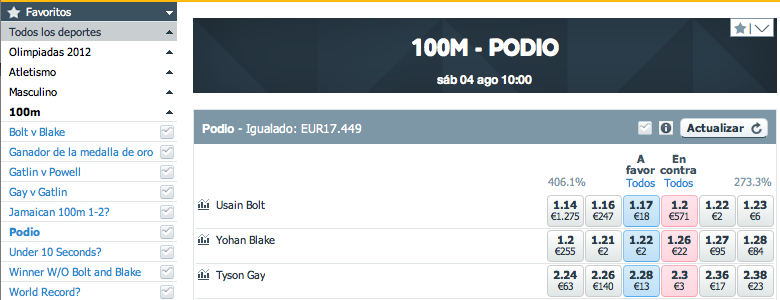
\includegraphics[width=0.95\linewidth]{./images/introbetfair.png} 
  \caption{Ejemplo de eventos y mercados en Betfair}
  \label{fig:eventoymercado}
\end{figure}

 Dentro del evento Olimpiadas, tenemos disponible el evento de los 100 metros lisos y la información del mercado acerca del ganador de la final.
 
\section{Apple y su terminal móvil \emph{iPhone}}
 
Apple Computer, Inc. es una empresa estadounidense de tecnología informática fundada en 1976. Inició sus trabajos sobre los ordenadores personales en la década de los setenta con el ordenador Apple II y reinventó el ordenador personal en los ochenta con el Macintosh. Hoy en día, Apple es considerada como una de las principales empresas líderes en tecnología.

El 9 enero del año 2007 presenta su primer terminal móvil llamado \emph{iPhone}. Tal y como lo hizo años atrás en la industria musical, su terminal se hizo famoso en la industría de la telefonía móvil por su diseño, su sistema operativo \emph{iPhone OS} y la introducción de nuevas tecnologías como la pantalla táctil.

\begin{figure} [h]
  \centering
    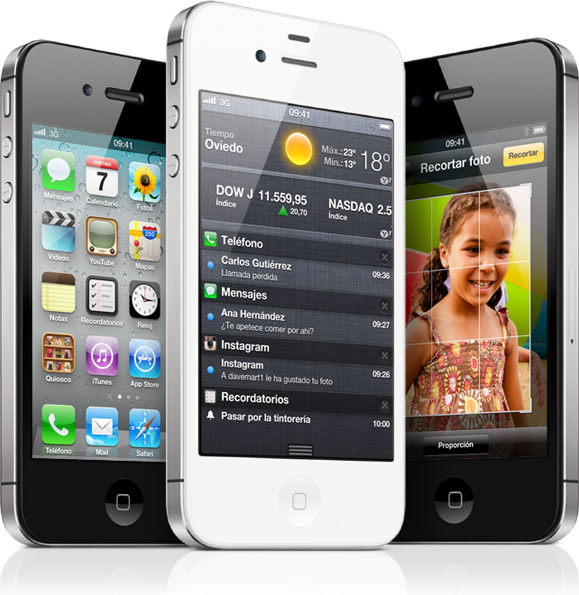
\includegraphics[width=0.6\textwidth]{./images/iphone4.jpg} 
  \caption{\emph{iPhone} 4S}
  \label{fig:iPhone-4GS}
\end{figure}
  
  En marzo de 2008 Apple muestra una nueva versión del terminal con tecnología 3G y comunica el lanzamiento de su propia tienda de aplicaciones para el \emph{iPhone}, la \emph{iTunes application store}. Para nutrir esa tienda de aplicaciones  lanza un conjunto de herramientas de desarrollo \emph{iPhone} \emph{SDK}\footnote{Software Development Kit} para todos aquellos desarrolladores que quieran participar en la misma. En el capítulo \ref{ch:diseno}  explicamos con más detalle dicho \emph{SDK} ya que es una pieza clave en el presente trabajo de fin de carrera.
  
   Otro hito importante a destacar ocurre el 27 de enero de 2010. Apple amplía la familia de dispositivos con una tableta táctil de 10 pulgadas denominada \emph{iPad}. Misma filosofía pero ahora en formato de pantalla más grande. De la misma forma que evoluciona sus dispositivos, evoluciona el \emph{SDK} para ofrecer a los desarrolladores las herramientas necesarias para crear aplicaciones compatibles entre la familia de dispositivos. A partir de 2010 el sistema operativo de los dispositivos para a denominarse \emph{iOS}. 
    
  Hoy en día, Apple dispone de un catálogo de más de 500.000 aplicaciones disponibles en su tienda\footnote{Fuente: www.apple.com y http://148apps.biz/app-store-metrics/} y más de 316 millones de terminales vendidos por todo el mundo.\footnote{Fuente: www.apple.com} He aquí la importancia de la temática de este trabajo de fin de carrera, adaptar el acceso de los servicios de Betfair a una de las plataformas móviles más extendidas del mundo.     
   
\section{Objetivos}

 El objetivo que se pretenden cubrir con el actual trabajo de fin de carrera es el acceso a los servicios web de Betfair a través de la plataforma \emph{iOS} de Apple. Para ello hemos marcado una serie de hitos a alcanzar:
 \begin{itemize}
 	\item Explorar y adaptar el \emph{API} de Betfair para la plataforma \emph{iPhone}.
 	\item Posibilidad de navegar y apostar por eventos del portal betfair.com a través del terminal móvil.
	\item Asesorar al usuario sobre cuando realizar el \emph{trading} a las apuestas ya realizadas.
\end{itemize}

%%% Local Variables: 
%%% mode: latex
%%% TeX-master: "tfc-betfair-ios"
%%% TeX-PDF-mode: t
%%% ispell-local-dictionary: "castellano"
%%% End: 

\cleardoublepage
%%%%%%%%%%%%%%%%%%%%%%%%%%%%%%%%%%%%%%%%%%%%%%%%%%%%%%%%%%%%%%%%%%%%%%%%
\chapter{REQUISITOS}
\label{ch:requisitos}
En este capítulo se presentan los requisitos a cumplir por la aplicación. Comenzaremos explicando el escenario al que pertenece la aplicación y terminaremos presentando las historias de uso de la misma.
\section{Escenario}

En el contexto de este trabajo de fin de carrera, un escenario es una descripción concreta del comportamiento de la aplicación en una determinada situación. El escenario general que se pretende cubrir con la aplicación es la posibilidad de navegar y realizar apuestas sobre eventos deportivos del portal Betfair.com. Se pretende cubrir las funcionalidades básicas que ofrece Betfair en su portal web para poder realizar apuestas y la posibilidad de realizar \emph{tranding} en las apuestas realizadas.

\section{Historias de usuario}
 Una de las formas de describir los requisitos es mediante la técnica de historias de uso. Son una representación de un requisito de software en una o dos frases usando un lenguaje común al usuario.
 
\subsection{Instalación} Para poder instalar la aplicación sólo se necesitará una cuenta del programa iTunes Store de Apple. La aplicación estará disponible para su descarga dentro de la tienda de aplicaciones  \emph{App Store} del dispositivo.  Alternativamente se podrá descargar también desde el programa iTunes para Windows y Mac. 
\subsection{Actualizar la aplicación}
La aplicación  \emph{App Store}  del dispositivo será la encargada de comunicar al usuario la aparición de una nueva versión del aplicativo. Para actualizarla simplemente habrá que seguir las indicaciones de dicho programa. %\fxnote{Lo mismo  de antes}

\subsection{Desinstalar}
Para desinstalar la aplicación simplemente se mantiene pulsado el icono de la misma unos segundos hasta que el icono empiece a vibrar. Inmediatamente pulsamos sobre el botón \textsf{X} que aparecerá es la esquina superior izquierda del icono de la aplicación. 
\subsection{Ejecución}
Para lanzar la aplicación sólo hay que pulsar el icono que aparece en la pantalla principal del dispositivo.
\subsection{Configurar la aplicación}
Se podrán configurar los diferentes aspectos de la aplicación tales como el idioma o las credenciales de acceso del  usuario a través del menú de ajustes del dispositivo. 
\begin{figure}[H]
    \centering
       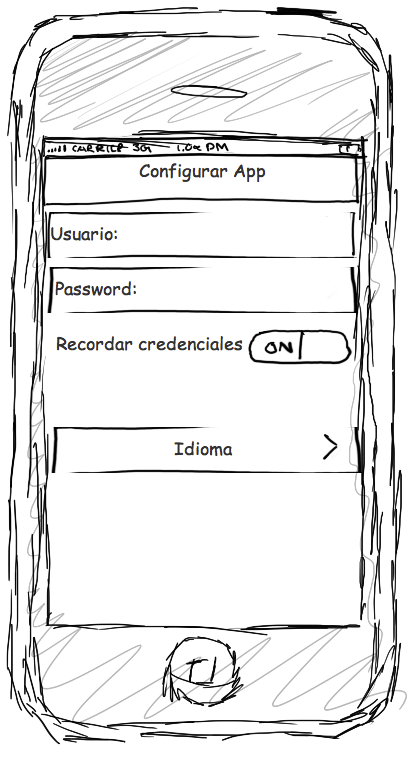
\includegraphics[width=0.3\textwidth]{./images/req_conf_app.png}
   \label{fig:Requisito configurar la aplicación}
\end{figure}
\subsection{Gestión de los eventos}
Se podrá navegar y obtener información de todos los eventos deportivos disponibles del portal Betfair. La aplicación ha de representar la información a través una jerarquía descendiente desde eventos hacia mercados de Betfair siguiendo las hojas de estilo de la interfaz de usuario de Apple.
\begin{figure}[H]
    \centering
       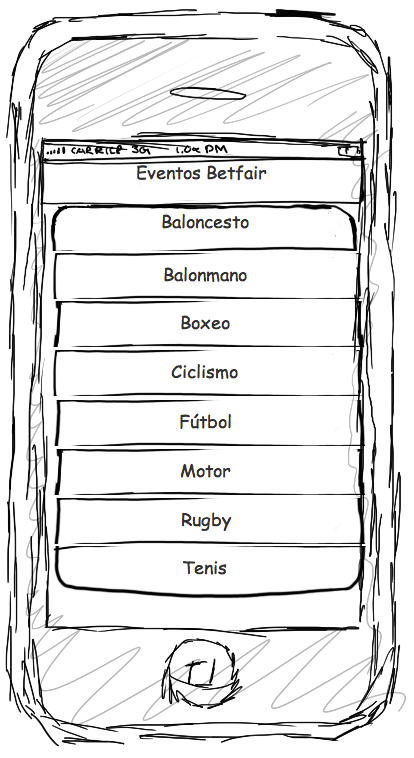
\includegraphics[width=0.3\textwidth]{./images/req_eventos.png}
   \label{fig:Requisito eventos}
\end{figure}
\subsection{Realizar una apuesta}
La aplicación permitirá la realización de una apuesta sobre un mercado específico incluyendo la cantidad y cuota deseada. El sistema notificará al usuario el resultado de la operación.
\begin{figure}[H]
    \centering
       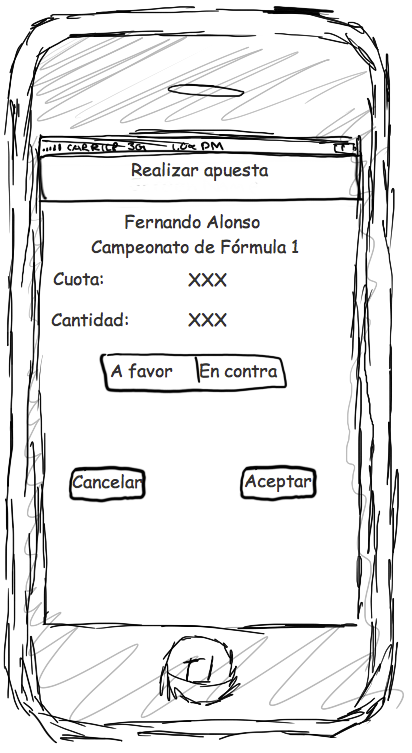
\includegraphics[width=0.3\textwidth]{./images/req_apuestas.png}
   \label{fig:Requisito realizar una apuesta}
\end{figure}
\subsection{Gestionar las apuestas}
La aplicación será capaz de recopilar todas las apuestas realizadas por el usuario sobre Betfair. Por cada apuesta, el sistema mostrará la información detallada de la apuesta, asesoramiento para \emph{trading} y estado actual del mercado.
\begin{figure}[H]
    \centering
       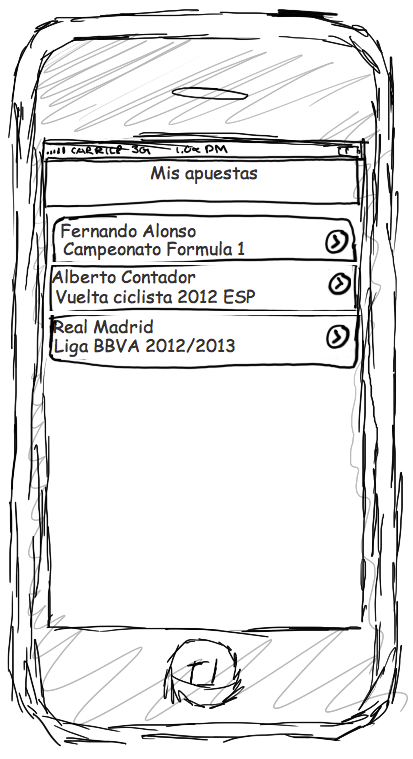
\includegraphics[width=0.3\textwidth]{./images/req_misapuestas.png}
   \label{fig:Requisito gestionar mis apuestas}
\end{figure}
\subsection{Realizar \emph{trading} sobre una apuesta ya realizada}
El sistema será capaz de asesorar para realizar \emph{trading} sobre una apuesta ya realizada anteriormente. La aplicación recomendará la apuesta más asequible a las condiciones del mercado. Se  podrá configurar la aplicación para que el \emph{trading} se realice de manera automática.
\begin{figure}[H]
    \centering
       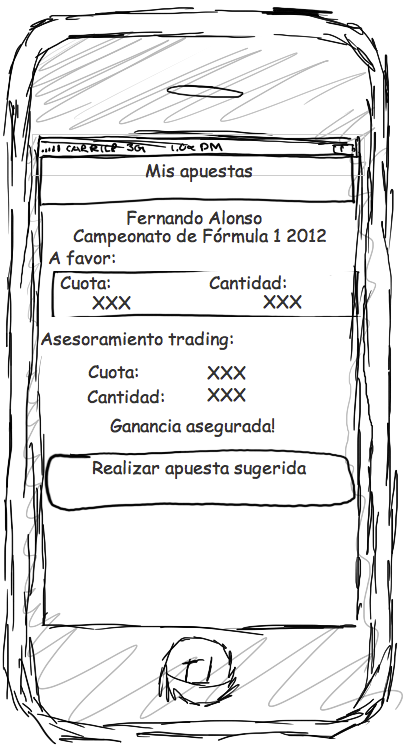
\includegraphics[width=0.3\textwidth]{./images/req_trading.png}
   \label{fig:Requisito trading}
\end{figure}

%%% Local Variables: 
%%% mode: latex
%%% TeX-master: "tfc-betfair-ios"
%%% TeX-PDF-mode: t
%%% ispell-local-dictionary: "castellano"
%%% End: 

\cleardoublepage
%%%%%%%%%%%%%%%%%%%%%%%%%%%%%%%%%%%%%%%%%%%%%%%%%%%%%%%%%%%%%%%%%%%%%%%%
\chapter{DISEÑO}
\label{ch:diseno}
 
  El análisis de los requisitos presentados en el capítulo \ref{ch:requisitos} dará como resultado la arquitectura de la aplicación. Para llevar a cabo su desarrollo, hemos tenido en cuenta la arquitectura del dispositivo y las herramientas adjuntas para el desarrollo de aplicaciones. Todas las decisiones tomadas en la construcción de la arquitectura de la aplicación se han basado en los límites o restricciones impuestas por el uso de la arquitectura de Apple y los límites impuestos en el uso del \emph{API} de Betfair. Para comprender mejor el diseño de la aplicación expondremos brevemente la arquitectura impuesta por Apple en el \emph{iPhone} y la tecnología en la que se basa el \emph{API} que ofrece Betfair para el uso de sus servicios.

\section{API de iOS: Cocoa Touch}
 La arquitectura del terminal móvil se basa en su sistema operativo \emph{iOS} de Apple. Este sistema operativo, a grandes rasgos, es un subconjunto del sistema operativo que llevan los ordenadores personales de Apple. Esta decisión favorece el desarrollo de aplicaciones para sus plataformas. Simplifica la tarea a los desarrolladores de aplicaciones de ordenadores de sobremesa de Apple de programar aplicaciones móviles sin necesidad de aprender un lenguaje o arquitectura totalmente nueva.
 
 %\fxnote{La introducción de gráficos o figuras puede hacerse de dos
  % formas: o la ``empotras'' directamente como he hecho yo con la
   %figura de las capas del OS o la metes en un entorno ``figure'' y la
   %referencias con un ``ref'' como he hecho con la figura \ref{fig:API
    % Betfair}, lo que creas más conveniente}

\noindent
La siguiente figura muestra la estructura en forma de capas en las que se compone el sistema operativo \emph{iOS}:

%\begin{center}
%  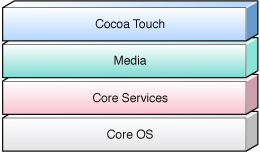
\includegraphics[width=0.5\textwidth]{./images/overview_systemlayers.jpg}
%\end{center}

\begin{figure} [h]
  \centering
    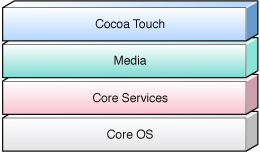
\includegraphics[width=0.5\textwidth]{./images/overview_systemlayers.jpg}
  \caption{Capas del \emph{iOS}}
  \label{fig:Capas-del-iOS}
\end{figure}

En la parte baja del sistema se encuentran las capas encargadas de los
servicios fundamentales que permiten la ejecución de las aplicaciones,
y en las superiores contienen las capas sobre los servicios multimedia
y de las más altas tecnologías.
 

A continuación expondremos una breve descripción de cada capa:

%\fxnote{He cambiado el entorno ``itemize'' a ``description'' para que
 % veas como queda, si te gusta lo mantienes, si no lo cambias. También
 % he modificado la indentación en el código fuente de latex para que
 % veas que se pueden meter cambios de linea sin probleamas (dos
 % cambios de linea consecutivos = nuevo párrafo).}

\begin{description}
\item[Core OS.]  Es la capa que contiene el núcleo de
  sistema (\emph{kernel}) %\fxnote{Recuerda, inglés enfatizado, al
   % menos en la primera aparición, encárgate tú del resto.},
  , los controladores para dispositivos internos y las interfaces básicas del sistema
  operativo. El \emph{kernel} es el responsable de todos los aspectos
  relacionados con el sistema operativo. Es el encargado de gestionar
  la memoria virtual, \emph{threads} (procesos ligeros), sistema de ficheros,
  red y procesos de comunicación. Los controladores son los encargados
  de proporcionar la interfaz entre el \emph{hardware} y los \emph{frameworks} de
  las capas superiores.
\item[Core Services.] Es la capa responsable de proporcionar los
  servicios básicos del sistema a las aplicaciones para su uso. En
  ella encontramos el acceso a la agenda del dispositivo, la gestión
  de estructura de datos, la gestión de las interfaces de red, la
  gestión de la localización del dispositivo, la gestión de la seguridad
  del sistema y el soporte para bases de datos \emph{SQL} y \emph{XML}.
\item[Media.] Es la capa encargada de dar soporte a las
  tecnologías de gráficos y al audio y video para proporcionar al usuario
  los medios multimedia vistos en un dispositivo móvil.
\item[Cocoa Touch.]  Es una de las capas más importantes del \emph{iOS}
  para un desarrollador de aplicaciones móviles. Se encarga de las interacciones del usuario con la interfaz táctil del dispositivo. 
 \end{description}
  
  Esta última capa es la que diferencia la plataforma móvil de la plataforma \emph{PC} en los entornos de Apple. Una vez visto lo esencial del sistema operativo \emph{iOS}, Apple nos proporciona en su \emph{API} un conjunto de \emph{frameworks}\footnote{Un framework es una estructura de soporte definida, en la cual otro proyecto de software puede ser organizado y desarrollado.} para poder acceder a las capas vistas anteriormente. Los más importantes son:  

 \begin{description}
 	\item [UIKit.] Contiene todas las clases necesarias para la programación de la interfaz de usuario de las aplicaciones así como el acceso a las principales tecnologías hardware 
	 propias del dispositivo  móvil. Es la más importante de todos los \emph{framework} ya que haciendo uso de ella crearemos la interfaz de usuario de nuestra aplicación:
		 \begin{itemize}
		  	\item soporte para la creación de gráficos y ventanas del sistema.
			\item soporte para la gestión de eventos \emph{multitouch} y eventos realizados al pulsar la pantalla con más de un dedo.
			 \item soporte para la creación de contenido tanto de texto como de web.
 			\item soporte para la creación de controles y objetos del sistema.
 			\item soporte para copiar, cortar y pegar.
 			\item soporte para la accesibilidad de aplicaciones.
 			\item soporte para el acceso a las capacidades hardware del dispositivo: batería, cámara, acelerómetros, sensor de proximidad \ldots 
 		\end{itemize}
 	 \item [Foundation.] Es un \emph{framework} heredado de la plataforma \emph{OS X}. Provee el soporte para las siguientes funcionalidades: 
 		\begin{itemize}
			\item colecciones de datos (arrays, sets \ldots)
			\item gestión del tiempo y fechas.
			\item gestión de las preferencias del dispositivo.
			\item gestión de URLs.
			\item internacionalización del dispositivo.
		\end{itemize}
	\item [Address Book UI.] Una de las partes más usadas en un dispositivo móvil es la agenda de contactos. Nos proporciona las herramientas necesarias para acceder a los contactos del dispositivo: crear, modificar, eliminar \dots
	\item [Message UI.] Proporciona el soporte necesario para componer y gestionar mensajes de correo electrónico o \emph{SMS} en nuestras aplicaciones.
	\item [Map kit.]  Esta interfaz proporciona la creación de una vista de un mapa geográfico escalable con posibilidad de incrustar en él información detallada. Un típico ejemplo es la localización en un mapa de un restaurante.
	\item [Push Notification Service.] Proporciona un camino para notificar a los usuarios que una aplicación tiene nueva información relevante. El sistema notifica al usuario la información incluso si la aplicación no está en ejecución.

\end{description}

 Para poder desarrollar aplicaciones para dispositivos \emph{iOS}, Apple pone a disposición de forma gratuita un conjunto de herramientas de desarrollo (\emph{SDK}) que se encuentra disponible en su portal web. 

\section{Arquitectura del \emph{API} de Betfair}

	Los servicios web que nos proporciona el \emph{API} de Betfair están diseñados bajo un protocolo \emph{SOAP}\footnote{Simple Object Access Protocol}. \emph{SOAP} es un protocolo estándar que define cómo dos objetos en diferentes procesos pueden comunicarse por medio de intercambio de mensajes, en este caso codificados en \emph{XML}\footnote{Extensible Markup Language, es un metalenguaje extensible de etiquetas desarrollado por el World Wide Web Consortium (\emph{W3C}).}. A continuación explicaremos qué son y cómo funcionan los servicios web para más adelante comprender las decisiones tomadas en la arquitectura de la aplicación.
	%\fixme{Esto hay que solucionarlo mediante una referencia bibliográfica utilizando bibtex, pregunta si no sabes cómo y lo vemos juntos.} 

%\fixme{Creo que se hace fundamental explicar en qué consiste todo este asunto del WSDL, cómo se usa (probablemente hay varios ``workflows'' posibles), un par de ejemplos pueden ser determinantes para entender la filosofía. En estos %momentos, como lector, estoy más interesado en que me cuentes cómo se materializa ese API que en ningún otra cosa. También puedes dar el ejemplo un poco más adelante y avisar al lector. Puedes utilizar subsections para organizar %bien la exposición.}

\subsection{Servicios web}

         Un servicio web es una interfaz de software que describe un conjunto de servicios u operaciones a las cuales se puede acceder por la red. El acceso a dichos servicios se realiza a través de intercambios de mensajes estandarizados. Para su comunicación usa protocolos basados en el lenguaje \emph{XML} con el objetivo de describir una operación para ejecutar o datos para intercambiar con otro servicio web.  
 
\begin{figure} [h]
  \centering
    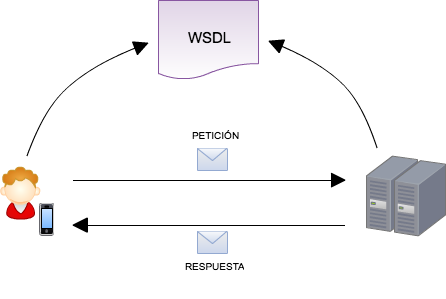
\includegraphics[width=0.6\textwidth]{./images/webservice.png}
  \caption{Funcionamiento servicios web}
  \label{fig:servicioweb}
\end{figure}
         
         Según el ejemplo de la figura \ref{fig:servicioweb}, un cliente, a través de una aplicación, realiza una petición de uso de un servicio web a través de un mensaje que ofrece un proveedor a través de Internet. El proveedor responderá a la petición con la información requerida en un mensaje con destino el cliente. En todo este proceso intervienen una serie de tecnologías que hacen posible esta circulación de información. Por un lado, estaría \emph{SOAP}. Se trata de un protocolo basado en \emph{XML}, que permite la interacción entre varios dispositivos y que tiene la capacidad de transmitir información compleja. Los datos son transmitidos a través de \emph{HTTP}\footnote{Hypertext Transfer Protocol}, es el método más común de intercambio de información en la web, el método mediante el cual se transfieren las páginas web a un ordenador. 
          Por otro lado, \emph{WSDL}\footnote{Web Services Description Language} permite que un servicio y un cliente establezcan un acuerdo en lo que se refiere a los detalles de transporte de mensajes y su contenido, a través de un documento procesable por dispositivos. \emph{WSDL} representa una especie de contrato entre el proveedor y el que solicita. \emph{WSDL} especifica la sintaxis y los mecanismos de intercambio de mensajes.
                    
 \subsection{Servicios web de Betfair }
 	El \emph{API} de Betfair está disponible a partir de un fichero en formato \emph{WSDL} en el portal de desarrolladores de Betfair. Dicho formato describe la interfaz para todos los servicios web disponibles de Betfair. En el capítulo \ref{ch:implemetacion} describiremos cómo hemos hecho uso de este fichero para construir las llamadas al servidor y consumir dichos servicios de Betfair.

 Los servicios web proporcionados por el \emph{API} de Betfair se dividen en dos conjuntos: 
          
\begin{itemize}
	\item \emph{Global}: contiene todas las llamadas referentes a los servicios básicos de Betfair, tales como el inicio de sesión, la administración de tu cuenta Betfair, tus fondos y las llamadas para navegar por los diferentes eventos disponibles en el portal de apuestas. 
	\item \emph{Exchange}: contiene las llamadas a los servicios relacionados con las apuestas, es decir, apostar por un evento, descripción de los mercados disponibles, actualización o cancelación de las apuestas ya realizadas, historial de todas nuestra apuestas\ldots 
\end{itemize}

  Para cada conjunto existen dos formas de acceso al \emph{API}:
\begin{description}
	\item [Free Access API.]  Con este acceso tendremos disponibles los servicios básicos del portal y las herramientas suficientes para poder apostar por los eventos disponibles. Es gratuito pero no contiene todos los servicios que proporciona Betfair.
	\item [Full Access API.] Acceso de pago donde están disponibles todos los servicios exclusivos del portal tales como la gestión de acceso a nuestro medio de pago de nuestra cuenta de usuario\ldots Se gestiona a partir de una cuota anual y no existen límites en las llamadas a los servicios del \emph{API}.
\end{description}

Resaltar en este apartado que dado que nuestra aplicación no soporta la plataforma \emph{WSDL}, hubo que implementar cada llamada a los servicios de Betfair bajo la tecnología de Apple y su posterior serialización para el tratamiento de datos de la aplicación. Por cada llamada descrita en el archivo de definición de servicios hemos tenido que implementar la estructura de la comunicación mediante mensajes \emph{XML}, uno de petición y otro de respuesta con un \emph{parser} asociado que traduzca dichos mensajes. En el capítulo \ref{ch:implemetacion} veremos con más detalle la adaptación de \emph{WSDL} a la plataforma \emph{iOS}.

\subsection{Servicios básicos necesarios}

    Los servicios básicos que hemos usado para el cumplimiento de los requisitos de la aplicación han sido:

\begin{itemize}
	\item \lstinline{Login}: 
		llamada para poder usar los servicios web de Betfair. 
	\item \lstinline{GetActiveEventTypes}: 
		con esta llamada obtenemos todos los eventos deportivos actualmente en marcha por los que se puede apostar.
	\item  \lstinline{GetAllMarkets}:
		con esta llamada obtenemos todos los mercados referentes a un evento.
	\item  \lstinline{GetCurrentsBets}:
		llamada por la cual obtenemos todas las apuestas activas que hemos realizado.
	\item  \lstinline{GetMarketPrices}:
		obtenemos los precios (\emph{back} y \emph{lay}) actuales por un evento determinado.
	\item  \lstinline{GetMarket}:
		esta llamada nos devuelve todos los datos referentes a un mercado.
	\item  \lstinline{PlaceBets}:
		con esta llamada enviamos una apuesta a Betfair.
	\item  \lstinline{ViewProfile}: 
		esta llamada nos devuelve los datos de perfil de usuario.
	\item  \lstinline{RetrieveLIMBMessage}:
		 con esta llamada obtenemos los mensajes del sistema pendientes de acción por parte del usuario.
\end{itemize}

\section{Arquitectura de la aplicación}

%\fixme{Averiguar a qué modelo MVC más se parece lo que has hecho y hablar de él a un nivel similar al que lo hace Fowler en http://martinfowler.com/eaaDev/uiArchs.html,  http://aspiringcraftsman.com/2007/08/25/interactive-application-architecture/ o http://www.codeproject.com/Articles/42830/Model-View-Controller-Model-View-Presenter-and-Mod}

 Para el diseño de la arquitectura nos hemos basado en el patrón de diseño ``Modelo Vista Controlador (\emph{MVC})'', exactamente Modelo Vista Controlador de \emph{Smalltalk}. Dicho patrón es muy utilizado en la programación orientada a objetos, donde los objetos del modelo representan los datos de la aplicación y son persistentes. Fundamentalmente consiste en separar los datos de una aplicación, la interfaz de usuario, y la lógica de control en tres componentes distintos:

 \begin{description}
 	\item [Modelo.] Es la representación de toda la información con la cual el sistema trabajará. El modelo es independiente de cualquier representación o vista.
	\item [Vista.] Se encarga de presentar el modelo en un formato adecuado para interactuar, normalmente mediante una interfaz de usuario.
	\item [Controlador.] Se encarga de responder a eventos. Esto implica cambios en el modelo y en la vista.
\end{description}
 
  La razón del uso de este patrón se debe a dos cuestiones fundamentales:
\begin{itemize}
	\item La facilidad entre la comunicación del modelo de datos y entre la interfaz. Cualquier cambio en la interfaz de usuario no afecta al resto del modelo, por lo que se gana en facilidad a la hora de seguir desarrollando la solución en el futuro.
	\item Apple, en el uso de las herramientas de desarrollo del \emph{SDK}, recomienda el uso de dicho patrón para la creación de la interfaz de usuario de la aplicación. Esta recomendación es debido a la arquitectura interna del \emph{iOS} y a que sus herramientas de desarrollo también están orientadas a esta solución.
	\item La estructura jerárquica de los datos obtenidos a través del \emph{API} de Betfair. Este patrón nos facilita la representación de los mismos.
\end{itemize}

%\fxnote{MVC es un nombre demasiado genérico y bastante manido, quizás quieras explorar con más profundidad las características exactas del patrón que hayas aplicado: http://www.aspiringcraftsman.com/2007/08/interactive-application-architecture/, http://c2.com/cgi/wiki?MvcIsNotObjectOriented}

\subsection{Núcleo de la aplicación}
	Toda aplicación para \emph{iOS} se desarrolla usando principalmente el \emph{framework} UIKit. UIKit proporciona todo lo necesario para lanzar la aplicación, coordinar los \emph{inputs} del usuario y mostrar el contenido en la pantalla. 
	Desde que el usuario pulsa el icono de la aplicación hasta que esta es ejecutada , el \emph{framework} UIKit gestiona todo lo necesario para lanzar la infraestructura. Toda aplicación recibe principalmente eventos continuamente desde el sistema y debe responder a todos estos eventos. 
	
	El ciclo de una aplicación esta formado por la secuencia de eventos del sistema:  pulsación en la pantalla por parte del usuario, llegada de un mensaje de texto\ldots que ocurren entre la ejecución y la finalización de la aplicación. En \emph{iOS}, el usuario lanza la aplicación pulsando sobre el icono de la misma en la pantalla.  A partir de este momento, UIKit es el encargado de lanzar la interfaz de usuario y de leer los eventos que se produzcan en un bucle hasta que la aplicación sea finalizada bien por el sistema o bien por el usuario. Durante el bucle, UIKit coordina la llegada de eventos a los objetos (el usuario pulsa una parte de la pantalla) y coordinar las respuestas de las mismas, es decir, qué hacer ante la acción del usuario. 
	     
 \begin{figure} [h]
  \centering
    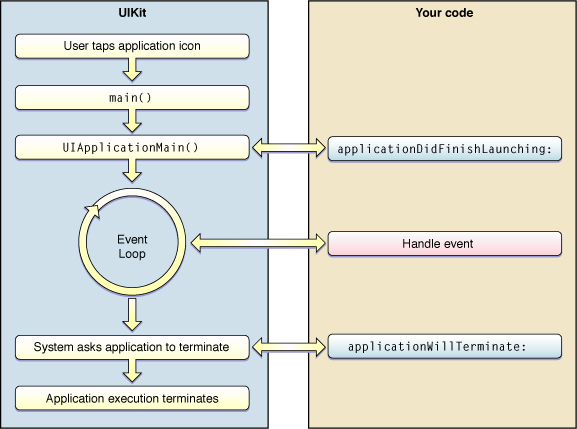
\includegraphics[width=0.8\textwidth]{./images/app_life_cycle.jpg}
  \caption{Ciclo de una aplicación \emph{iOS} }
  \label{fig:iOS-layers}
\end{figure}
     
   La figura \ref{fig:iOS-layers} muestra el ciclo de una aplicación para \emph{iOS}. Tal y como vemos, UIKit se encarga del arranque de la aplicación y de la gestión de eventos. Nuestro código será el encargado de gestionar esos eventos cuando reciba la notificación de que la aplicación ha sido lanzada. También podremos gestionar las accionas oportunas (guardar preferencias o cambios producidos en la aplicación) cuando UIKit nos notifique la finalización de la aplicación.
   
    En \emph{iOS} sólo se finaliza una aplicación por tres motivos:
    \begin{itemize}
	\item El usuario finaliza la misma pulsando el botón \textsf{Home}. 
	\item El sistema recibe una notificación prioritaria que atender, una llamada por ejemplo, y por tanto finaliza la aplicación.
	\item El sistema detecta un comportamiento erróneo de la aplicación y para salvaguardar la estabilidad del sistema finaliza nuestra aplicación.
     \end{itemize}

 \begin{figure} [h]
  \centering
    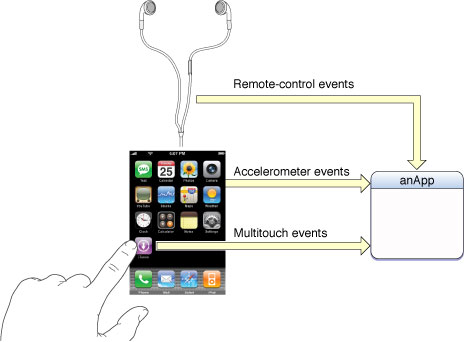
\includegraphics[width=0.8\textwidth]{./images/events_to_app.jpg}
  \caption{Notificaciones del sistema \emph{iOS} }
  \label{fig:iOSnotify}
\end{figure}

 La figura \ref{fig:iOSnotify} muestra un ejemplo de las notificaciones que puede recibir una aplicación por parte del sistema.
 
    Es responsabilidad del desarrollador asociar a cada evento un método adecuado para gestionarlo. Si el desarrollador deja un evento sin asociar, la aplicación simplemente lo ignorará. En nuestra aplicación, gestionamos acciones antes las siguientes notificaciones:
    
\begin{itemize}
	\item \lstinline{didFinishLaunchingWithOptions}: El sistema nos indica que nuestra aplicación ha sido lanzada y tomamos el control a partir de ese momento. 
 	\item \lstinline{applicationWillTerminate}: El sistema nos indica que finalizará nuestra aplicación para salvaguardar la estabilidad del sistema. Básicamente guardaremos el estado de la aplicación.
	\item \lstinline{applicationDidEnterBackground}: El sistema nos indica que nuestra aplicación pasa a segundo plano. Guardaremos el estado de la aplicación y suspenderemos cualquier acción que este en curso.
\end{itemize} 
    
%\fixme{Dudas que me surgen y que no se si este es el sitio o el momento adecuado para resolverlas. Lo que sí se es que impactan en el diseño: ¿qué eventos llegan al ``Your code''? ¿Qué reglas existen para tratarlos? ¿Se enlazan los eventos a métodos? ¿Se puede modificar ese supuesto ``vector de interrupciones''? ¿Los eventos son independientes de los objetos gráficos? Seguro que contestas a estas preguntas más adelante pero a mi, como lector, me gustaría saber algo más ahora.}    
    
\subsection{Controladores de Vista}	   
 
 Un controlador de vista del \emph{SDK} proporciona la lógica básica de interfaz de usuario para dibujar las vistas de la aplicación. Definimos como vista de usuario la pantalla que se le presenta en un momento dado. El sistema dispone de varios patrones de interfaces de usuario para ayudar a representar el conjunto de datos hacia el usuario en las aplicaciones dentro de los dispositivos móviles. 
 
  Un controlador de vistas gestiona la vista de nuestra aplicación que aparece entre las barras superiores e inferiores (véase figura \ref{fig:layout-of-views}).
  La vista de la aplicación aparece entre la barra de estado y la barra de navegación si ésta está presente. En una vista de aplicación se muestra una parte de datos y controles que el desarrollador quiere mostrar al usuario en un tiempo determinado. El controlador de la vista simplemente gestiona la presentación de esta vista y la siguiente en aparecer para un patrón de diseño establecido.
 
 \begin{figure} [h]
  \centering
    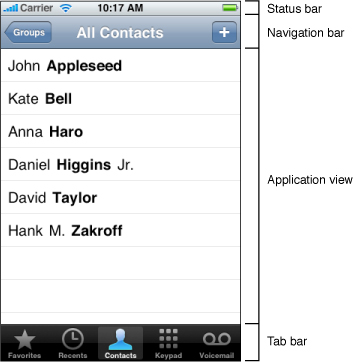
\includegraphics[width=0.6\textwidth]{./images/vc-areas.jpg}
  \caption{Esquema de las vistas }
  \label{fig:layout-of-views}
\end{figure} 
 
 Los controladores de vista nos ahorran código al automatizar la presentación de cada vista al usuario. Es decir, excluyen al desarrollador de tareas tan básicas como la presentación de los objetos en pantalla o la captura de los inputs del usuario. También ayudan al diseño orientado de objetos separando los detalles de la interfaz de usuario de la lógica de la aplicación.
  
 \subsection{Controlador Vista de tablas}	

  Es muy común usar vistas de tabla para mostrar un conjunto de datos de tipo jerárquico para poder recorrerlos.  
  Para ello, disponemos de un controlador específico llamado ``Controlador de vistas de tabla'' que nos proporciona todo lo necesario para su representación y gestión. En nuestra aplicación, tenemos que mostrar el modelo de datos que recogemos de los servidores de Betfair. Éstos están organizados de forma jerárquica, de lo más general a lo más específico. Recordemos que el modelo se basa básicamente en eventos y mercados, y que cada evento puede contener más eventos y mercados. Para poder realizar una apuesta en un partido de fútbol concreto antes hemos tenido que elegir deporte, categoría, país, división y finalmente el partido. La mejor forma de representarlos es mediante una vista de tabla tal y como nos recomiendan las hojas de estilo de Apple.
  
   En la figura \ref{fig:table-view-top} podemos ver un esquema representativo de la información más general. Este caso se podría representar los eventos más altos del modelo de datos de Betfair.
  
 \begin{figure}[h!]
  \centering
    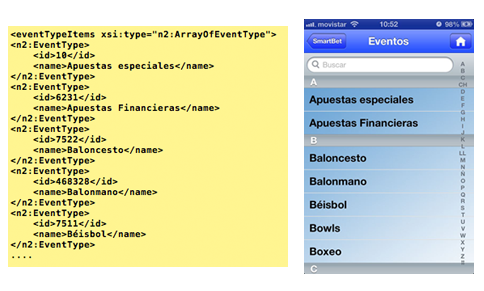
\includegraphics[width=0.8\textwidth]{./images/tabla_top.png}
  \caption{Vista de tabla del top de la jerarquía }
  \label{fig:table-view-top}
\end{figure} 

 En la figura \ref{fig:table-view-middle} nos encontramos una información de tipo jerárquica en la mitad de recorrido. Comparándolo con el modelo de Betfair sería la representación de eventos y mercados en la misma vista. Podemos asociarla al ejemplo de la elección de la división.

\begin{figure}[ht!]
  \centering
    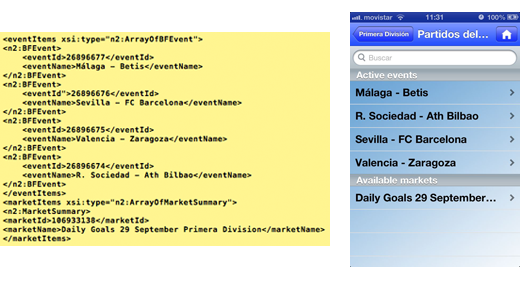
\includegraphics[width=0.8\textwidth]{./images/tabla_middle.png}
  \caption{Vista de tabla de la mitad de la jerarquía}
  \label{fig:table-view-middle}
\end{figure} 

 A continuación representamos el final de nuestro recorrido por el modelo de datos. Como podemos observar en la figura \ref{fig:detail-table-view}, hemos alcanzado la información más específica. Es nuestro caso, solo una lista de mercados disponibles de Betfair.

\begin{figure}[ht!]
  \centering
    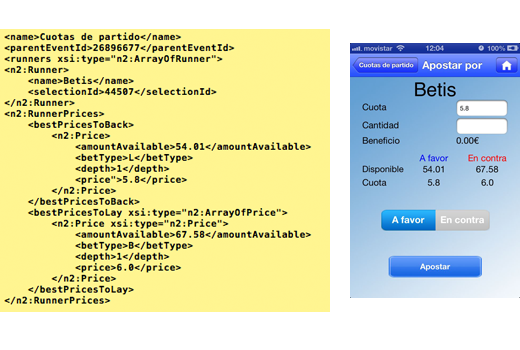
\includegraphics[width=0.8\textwidth]{./images/tabla_detail.png}
  \caption{Vista de tabla detallada del final de la jerarquía }
  \label{fig:detail-table-view}
\end{figure} 

\subsection{Arquitectura de la aplicación}	
   
   La aplicación esta formada principalmente por un conjunto de controladores de vista más un módulo encargado de comunicarse con el \emph{API} de Betfair. Como hemos visto anteriormente, hemos hecho uso de las herramientas del \emph{SDK} más adecuadas para navegar por la estructura de datos de Betfair. Para ello hemos creado diferentes controladores de vista para poder ofrecer al usuario la mejor vista para la representación de los datos en cada caso de uso.%\fixme{Fíjate que ésta es una decisión de diseño que aún no has explicado.}
   
   %\begin{figure} [h]
     %\centering
     %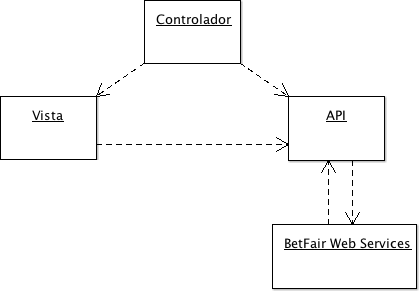
\includegraphics[width=0.8\textwidth]{./images/modelo1.png}
     %\caption{Esquema modelo vista controlador }
     %\label{fig:esquema-MVC}
   %\end{figure}
   
    %En la figura \ref{fig:esquema-MVC} podemos ver un esquema del modelo Vista Controlador usado. % \fxnote{de la arquitectura?}.
     %Los controladores de vista se encargan de recoger los eventos de la aplicación, principalmente \emph{inputs} del usuario. % \fxnote{eventos?}. 
     %En el caso de que el input involucre datos de Betfair, el controlador envía los datos necesarios para que el módulo de comunicación obtenga la respuesta por parte del API de Betfair. 
    
\subsubsection{Controlador principal}

 Es la clase principal de la aplicación. Es la encargada de iniciar el controlador de vista que será encargado de recoger los eventos del usuario, así como la gestión de memoria y la gestión de los eventos del sistema.
 
\subsubsection{Controlador de menú principal (RootViewController)}
 Es la encargada de mostrar las opciones principales del programa y recoger los inputs del usuario para lanzar el controlador adecuado a la elección del usuario. También se encarga de gestionar el inicio de sesión del usuario para los servicios web de Betfair. Para ello hace uso del servicio \lstinline{login} de Betfair a través de la clase de comunicación llamada \emph{API}.
 
 \subsubsection{Controlador de perfil de usuario (ViewProfileController)}
 Muestra al usuario una lista con toda la información registrada en su perfil de Betfair, tales como el nombre de usuario, información de contacto y límite de apuestas diaria. Hace uso del servicio de Betfair \lstinline{ViewProfile}  a través de la clase \emph{API} del modelo de la aplicación.
 
\subsubsection{Controlador de tipos de eventos (EventsTypeController)}
 Muestra al usuario una lista con todos los tipos de eventos activos por los que se puede apostar dentro de Betfair. En un futuro se podrá gestionar por fecha de finalización, orden alfabético o búsqueda directa de eventos. Una vez seleccionado el evento deseado, se lanza el controlador de eventos y mercados con la información relativa al evento previamente seleccionado. Hace uso del servicio de Betfair \lstinline{GetActiveEventsTypes}  a través de la clase \emph{API} del modelo de la aplicación.
 
\subsubsection{Controlador de eventos y mercados (EventsAndMarketsController)}

 Es la clase encargada de mostrar de forma jerárquica los subeventos y mercados relacionados con un evento seleccionado previamente en el controlador de eventos. Igualmente se podrá gestionar por fecha de finalización, orden alfabético o búsqueda directa de eventos. En caso de ser seleccionado un evento, se le mostrará los mercados y subeventos relacionados con los mismos. Si se selecciona un mercado se procederá a lanzar el controlador de información de mercado. Para ello recaba la información obtenida a través del servicio web \lstinline{GetEvents} de Betfair.
 
\subsubsection{Controlador de información de mercado (MarketInfoController)}

 Es el responsable de gestionar toda la información relevante al mercado en cuestión. Gestionará el estado del mercado y sus propiedades obteniendo todo lo necesario del portal de Betfair a través del \emph{API} de sus servicios web haciendo uso de las llamadas del \emph{API}:
 
  \begin{itemize}
	\item \emph{GetMarket}: obtiene todos los parámetros acerca del mercado.
	\item \emph{GetMarketPrices}: obtiene todos los precios actuales del mercado en cuestión.
\end{itemize}

\subsubsection{Controlador de apuesta por un mercado (PutBetController)}
 Gestiona todos los datos necesarios e introducidos por el usuarios para realizar una apuesta y enviarla a Betfair. El método usado para enviar la apuesta a Betfair a través de la clase interfaz de comunicación es \emph{PlaceBets}.

\subsubsection{Controlador de las categorías de Mis Apuestas (MyBetsCategoryController)}
 Es la clase encargada de gestionar las apuestas ya realizadas en Betfair y que siguen activas. Las clasifica por categorías de mercado. Recoge la información como resultado de las llamadas a los siguientes servicios web de Betfair:
  \begin{itemize}
	\item \emph{GetMarket}: obtiene todos los parámetros acerca del mercado de una apuesta en cuestión.
	\item \emph{GetCurrentBets}: obtiene todas las apuestas realizadas por el usuario del servicios Betfair.
\end{itemize}
 
\subsubsection{Controlador de Mis Apuestas (MyBetsController)}
 Esta clase se encarga de gestionar las apuestas realizadas por el usuario dentro de una categoría determinada. En ella se muestra resumidamente el nombre de la apuesta en cuestión, la cuota apostada y la cuota actualizada en ese momento. 

\subsubsection{Controlador de detalles de una apuesta (MyBetDetailsController)}
 Se encarga de gestionar los detalles más relevantes sobre una apuesta determinada: parámetros, \emph{stake}, apuesta a favor o en contra relacionadas con la presentada\ldots También incluye información completa del mercado actual referente al mercado de la apuesta y el \emph{trading} acerca de la misma.
 
 \subsubsection{Controlador de propiedades de una apuesta (MyBetsProperties)}
 Se encarga de mostrar al usuario todos los detalles asociados a una apuesta determinada. 

\subsubsection{Controlador de \emph{trading} (TradingController)}
  Se encarga de asesorar al usuario sobre realizar el método \emph{trading} sobre una apuesta ya realizada. 
  
\subsubsection{API: Interfaz a Betfair}
 Esta clase se encarga de gestionar las comunicaciones con los servidores de Betfair. Envía las peticiones a los servicios web de Betfair y se encarga de realizar la decodificación de la respuesta a dichas peticiones en un formato adecuado para la aplicación.

\subsubsection{Controlador Parser (ParserXML)}
 Es la clase encargada de estructurar los datos de envío o recepción del servicio web a una estructura de datos adecuada para la aplicación y para la comunicación con Betfair.

\section{Diagrama de Estructura \emph{UML}}
 En la figura \ref{fig:estructura} podemos ver el diagrama de la estructura del proyecto. Observamos que el núcleo principal de esta aplicación es la clase ``API''. Como bien hemos descrito, es la encargada de comunicarse con el servidor de Betfair tanto para enviar las peticiones como de procesar las respuestas. Esta clase necesita un \emph{parser} de \emph{XML} para procesar los datos tantos del mensaje de petición de servicio como del mensaje de respuesta. De esta tarea se encarga la clase ``ParserXML''.
 
  Las clases que rodean a ``API'' son todos los controladores de vista de la aplicación. Son los que reciben las peticiones de la vista y, según el caso, hacer uso de un servicio concreto de Betfair a través de la clase ``API''. ``RootViewController'' es la clase a la que el sistema le otorga el control una vez se ha lanzado la aplicación. Su principal función es procesar el menú principal.

 \begin{figure}[h!]
    \centering
       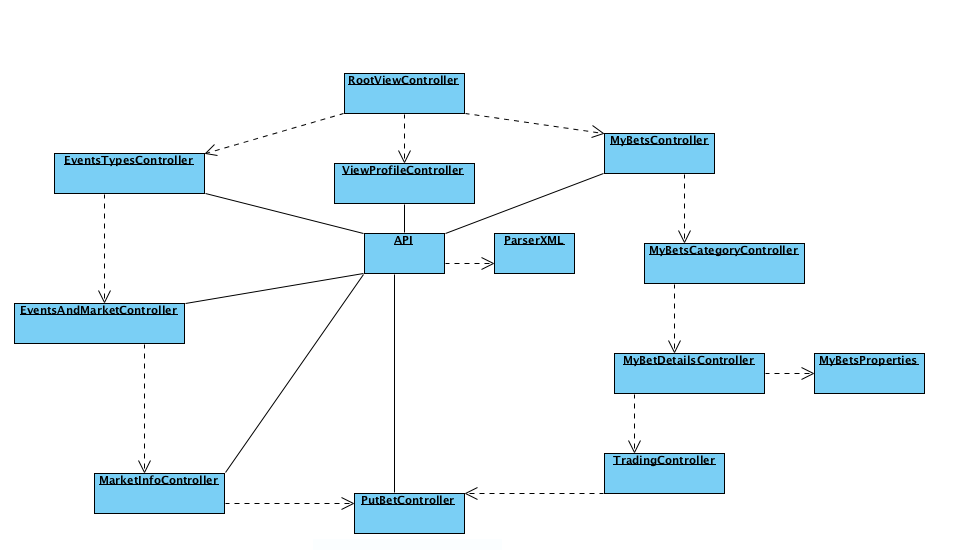
\includegraphics[width=0.95\linewidth]{./images/UML_Diagram.png}
     \caption{Diagrama de estructura \emph{UML}}
   \label{fig:estructura}
\end{figure}

%%% Local Variables: 
%%% mode: latex
%%% TeX-master: "tfc-betfair-ios"
%%% TeX-PDF-mode: t
%%% ispell-local-dictionary: "castellano"
%%% End: 

\cleardoublepage
%%%%%%%%%%%%%%%%%%%%%%%%%%%%%%%%%%%%%%%%%%%%%%%%%%%%%%%%%%%%%%%%%%%%%%%%
\chapter{Implementación}
\label{ch:implemetacion}
 En este capítulo se describirán todos los detalles relativos a la implementación de la aplicación. Empezaremos detallando el entorno de ejecución y el lenguaje de programación usado para su desarrollo y terminaremos destacando los detalles relevantes de la implementación. A saber:
 
\section{Entorno de ejecución}
 La aplicación desarrollada se ejecuta en un entorno llamado \emph{Cocoa Touch}. Cocoa es un conjunto de frameworks orientados a objetos que proporcionan un entorno de ejecución para las aplicaciones que se ejecutan en el sistema operativo \emph{iOS}. Este entorno de desarrollo nos facilita a los desarrolladores la tarea de pasar de la etapa de diseño a la etapa de desarrollo para crear una aplicación. \emph{Cocoa Touch} proviene del entorno de la plataforma \emph{Mac OS}, entorno de los que dependen los equipos de sobremesa de Apple. Se puede decir que es la misma plataforma añadiendo el soporte para los eventos táctiles y orientados a la tecnología móvil. 
 
 \emph{Cocoa} presenta dos caras: 
 \begin{itemize}
	\item Entorno de ejecución: las aplicaciones desarrolladas en Cocoa presentan la interfaz de usuario de la aplicación y están fuertemente integradas con otras partes del sistema operativo como por ejemplo el buscador del sistema de ficheros.
	\item Entorno de desarrollo: Cocoa es una suite de componentes software que están orientados a objetos y que te permiten rápidamente crear robustas y completas aplicaciones para el sistema operativo.
\end{itemize}
  
 \begin{figure}[ht!]
    \centering
       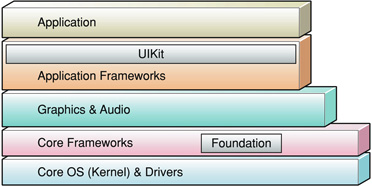
\includegraphics[width=0.9\textwidth]{./images/architecture_stack.jpg}
     \caption{Entorno \emph{iOS}}
   \label{fig:iOS Platform}
\end{figure}
 
 A pesar de que la estructura del \emph{iOS} es similar a la de la plataforma \emph{Mac OS}, existen diferencias significantes. El diagrama del \emph{iOS} muestra una plataforma como una serie de capas que van desde en núcleo de sistema operativo hasta un conjunto de frameworks de aplicación, la más crítica (para las aplicaciones) empieza con la capa UIKit.
 
 Para desarrollar en entornos \emph{Cocoa} se utiliza el lenguaje \emph{Objective-C}. Este lenguaje está basado en la programación orientada a objetos. Se define como un superconjunto del lenguaje de programación \emph{C}, es decir, podemos considerarle como una fina capa que complementa a \emph{C}. La sintaxis de objetos de \emph{Objective-C} deriva de \emph{Smalltalk}\footnote{Smalltalk es un lenguaje de programación que permite realizar tareas de computación mediante la interacción con un entorno de objetos virtuales.}.
 
  Como todo lenguaje de programación orientado a objetos, \emph{Objective-C} nos proporciona principalmente:
 \begin{itemize}
	\item Un lenguaje de programación orientado a objetos.
	\item Una extensa librería de objetos.
	\item Una conjunto software de herramientas de desarrollo.
	\item Un entorno de ejecución propio.
\end{itemize}

 Aparte de las características propias del lenguaje, al estar basado en el lenguaje \emph{C}, su compilador es capaz de ejecutar líneas de código codificadas en \emph{C}. Esta característica permite usar librerías realizadas en \emph{C} en programas desarrollados en \emph{Objective-C}.  En el presente trabajo hemos optado por usar el lenguaje \emph{Objective-C} en todo el desarrollo por ser el recomendado por Apple para una mejor integración con \emph{iOS}.
 
\section{Estructura de la aplicación}
 Cuando construimos una aplicación para el sistema operativo \emph{iOS} usamos la herramienta que nos proporciona el SDK de Apple \emph{Xcode}. Es un editor software que contiene todos lo necesario para compilar proyecto escrito en \emph{Objective-C}. La ventaja de usar este editor y no uno universal que acepte dicho lenguaje de programación es que \emph{Xcode} es capaz de implementar nuestra aplicación en lo que llamamos un paquete. Este paquete es un directorio en el sistema de ficheros que agrupa los recursos necesarios para la aplicación en un mismo lugar. Dicho paquete contiene el ejecutable y cualquier recurso usado por el mismo (por ejemplo, el icono de la aplicación, imágenes contenidas \ldots). El siguiente cuadro lista el contenido del paquete de esta aplicación.
 
\begin{center}
\tablefirsthead{\hline\hline\rowcolor[gray]{0.9}Archivo & Descripción\\\hline\hline}
\tablehead{\hline\hline\rowcolor[gray]{0.9}Archivo & Descripción\\\hline\hline}
% \tabletail{}
% \tablelasttail{}
\bottomcaption{Contenido de un paquete Xcode Cap}
\begin{supertabular}{||p{0.45\linewidth}|p{0.45\linewidth}||}
\lstinline!BetfairApp! & El fichero ejecutable de la aplicación. El nombre de este fichero es el mismo que el de la aplicación más la extensión app.\\ 
\hline 
\lstinline!Default.png! & Imagen de 480 x 320 píxeles que se muestra nada más iniciarse la aplicación  a modo de introducción. El sistema usa esta imagen mientras realiza tareas en segundo plano que requieren de un tiempo sensible para el usuario.\\
\hline
\lstinline!Settings.bundle! & Es un fichero que contiene las preferencias de la aplicación a personalizar por el usuario, como por ejemplo el lenguaje de la aplicación, el tipo de moneda a mostrar\ldots \\
\hline
\lstinline!iconBF.png! & Icono de 57 x 57 píxeles que representa la aplicación en la pantalla principal del dispositivo. \\
\hline
\lstinline!Info.plist! & También conocida como lista de propiedades. Este fichero es un lista donde se definen los valores claves de la aplicación tales como el identificador de aplicación, la versión y el título.\\
\hline
\lstinline!en.lproj! & Archivo que contiene los textos de la interfaz en inglés. Usado por el sistema cuando este lenguaje esta por defecto para lanzar aplicación o definido en las preferencias de la aplicación.\\
\hline
\lstinline!es.lproj! &Archivo que contiene los textos de la interfaz en español.\\
\hline
\lstinline!MainWindows.xib! & Contiene la interfaz a cargar por defecto por el sistema una vez lanzada la aplicación. Contiene la ventana principal de la interfaz de usuario. \\
\hline
\lstinline!RootViewController.xib! & Contiene los objetos necesarios de la interfaz de usuario del menú principal. \\
\hline
\lstinline!EventsControllerView.xib! &Contiene los objetos necesarios de la interfaz de usuario del menú de los eventos activos. \\
\hline
\lstinline!EventsTypesControllerView.xib! & Contiene los objetos necesarios de la interfaz de usuario de los tipos de eventos de Betfair. \\
\hline
\lstinline!EventsAndMarketsControllerView.xib! & Contiene los objetos necesarios de la interfaz de usuario de los eventos y mercados disponibles. \\
\hline
\lstinline!MarketInfoControllerView.xib! & Contiene los objetos necesarios de la interfaz de usuario de las características de un mercado. \\
\hline
\lstinline!PutBetControllerView.xib! & Contiene los objetos necesarios de la interfaz de usuario de la realización de una apuesta. \\
\hline
\lstinline!MyBetsControllerView.xib! & Contiene los objetos necesarios de la interfaz de usuario del menú de las apuestas ya realizadas por el usuario. \\
\hline
\lstinline!MyBetsCategoryController.xib! & Contiene los objetos necesarios de la interfaz de usuario de las categorías de apuestas realizadas por el usuario. \\
\hline
\lstinline!MyBetsDetailsView.xib! & Contiene los objetos necesarios de la interfaz de usuario con los detalles de una apuesta ya realizada y las opciones disponibles. \\
\hline
\lstinline!MyBetPropertiesView.xib! & Contiene los objetos necesarios de la interfaz de usuarios de los datos del mercados en los que se realizó la apuesta con las opciones posibles a realizar sobre esta. \\
\hline
\lstinline!TradingController.xib! & Contiene los objetos necesarios de la interfaz de usuario con los detalles acerca del trading sobre una apuesta. \\
\hline 
\hline 
\end{supertabular} 
\label{fig:componentes}
\end{center} 

\section{Internacionalización}
 Una parte importante a destacar en el proyecto es la posibilidad de establecer el idioma de la aplicación. Mediante la tienda de aplicaciones \emph{iTunes App Store} se puede distribuir la aplicación por diferentes países. Una aplicación de \emph{iOS} debe tener la posibilidad de poder mostrar varios idiomas y tener uno por defecto. Cada lenguaje esta implementado en la carpeta \emph{nombre-aplicación.lprj} del paquete de implementación ya comentado en el cuadro \ref{fig:componentes}. En el conjunto para proporcionar el soporte a distintos idiomas también se podrá especificar una imagen de portada, icono de la aplicación, mensajes de alerta\ldots  adecuado al idioma escogido por el usuario. Por defecto, el sistema operativo \emph{iOS} arranca la aplicación con los argumentos necesarios para que muestre la aplicación en el mismo idioma especificado en las preferencias del terminal, es decir, es el mismo lenguaje que esté configurado en éste. En caso de que no fuera posible, se procederá con el especificado por defecto de la aplicación.

  \begin{figure}[h!]
    \centering
       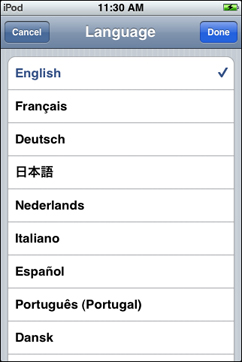
\includegraphics[width=0.5\textwidth]{./images/language.jpg}
     \caption{Ejemplo de la elección del idioma }
   \label{fig:Vista de las preferencias del idioma}
\end{figure}

 
  En esta implementación se procederá a dar soporte al español y al inglés, dos de los lenguajes más hablados dentro de la lista mundial.
  
  
  
  \begin{figure}[h!]
  	\centering 
  		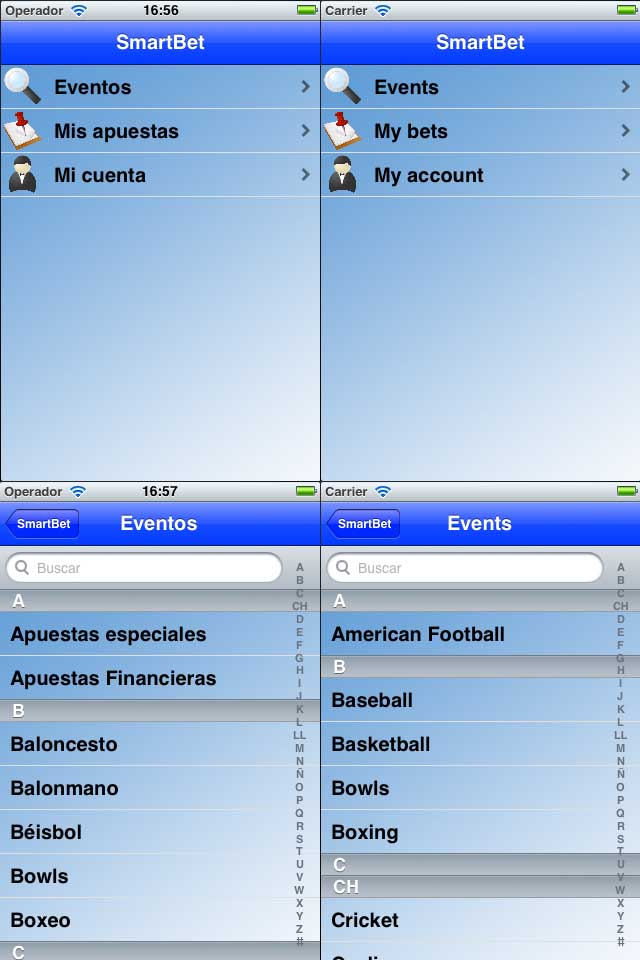
\includegraphics[width=0.7\textwidth]{./images/lenguajes.jpg}
	\caption{Ejemplo de interfaz con distinto idioma seleccionado.} 
	\label{fig:Ejemplo de interfaz con distinto idioma seleccionado.}
\end{figure} 
  
  
  
  Para implementar esta funcionalidad dentro de nuestro trabajo de fin de carrera hemos de definir la lista de palabras a traducir dentro de un archivo llamado \emph{Localizable.strings}.  Este archivo contiene una lista de la tupla etiqueta-traducción. El sistema, cada vez que encuentra una etiqueta en la interfaz de usuario la sustituye por la traducción del idioma en el que este configurado el terminal. A continuación se muestra un ejemplo del contenido de dicho fichero.
  
\begin{lstlisting}
/* 
   Localizable.strings
   Betfair App

   Created by Francisco on 21/12/11.
   Copyright 2011  . All rights reserved.
*/
"Events" = "Eventos";
"My bets" = "Mis apuestas";
"My account" = "Mi cuenta";
"Announcements" = "Mensajes del sistema";
"Profile" = "Cuenta";
"Bet info" = "Info. apuesta";
"Your bet" = "Tu apuesta";
"Nothing" = "Vacio";
"Active events" = "Eventos activos";
"Available markets" = "Mercados disponibles";
"Bet for" = "Apostar por";  
\end{lstlisting}

  
   Por ejemplo, para mostrar el título ``Mis Apuestas'' en español el sistema buscará la etiqueta en el archivo \emph{Localizable.string} perteneciente al idioma español. En el código especificaremos la etiqueta a mostrar ``My bets'' y el sistema, en tiempo de ejecución, mostrará su traducción, en este caso ``Mis apuestas''.  Este archivo se ubica dentro de la carpeta es.lpjr o en.lpjr según sea la tabla de traducción en inglés o en español. 
   
   Berfair, en su \emph{API} nos permite especificar en cada servicio en que idioma queremos recibir la respuesta. Con la combinación de ambas funcionalidades tenemos en el presente fin de carrera la aplicación completamente traducidas en dos idiomas disponibles: inglés y español. 
   
\section{Interpretación XML de Betfair a Cocoa Touch}
 Como ya tratamos en el capítulo \ref{ch:diseno}, un tema clave a destacar es la adaptación del \emph{API} de Betfair a la arquitectura del terminal iPhone. 
 
  Betfair ofrece el acceso a todos sus servicios a aquellos programadores que quieren incluirlos a través de aplicaciones. Es un camino eficaz para hacer llegar sus servicios a usuarios de otras plataformas o para usuarios expertos que requieran de una interfaz de usuario más experta, orientada a sus necesidades. Por supuesto que esta política requiere de un sistema de seguridad para evitar fraudes o ataque por parte de la comunidad de hackers.
   
  En el diseño de una aplicación que debe hacer uso de servicios web ofrecidos por un sistema externo se necesita algún tipo de \emph{API} o interfaz para acceder a los mismos. Lo primero a tener en cuenta es lo que se necesita para hacer uso de las funciones proporcionadas por el \emph{API}. Para acceder a los servicios ofrecidos por Betfair, como ya vimos en la figura \ref{fig:servicioweb} necesitamos conocer la interfaz de acceso que se describe  en un archivo en formato WSDL. Este tipo de archivo es muy común y se usa para describir interfaces públicas de acceso a servicios web. Está basado en XML y contiene los requisitos, parámetros y formatos de los mensajes necesarios para interactuar con los servicios disponibles. 
   
   Existen herramientas en el mercado que traducen de forma automática el archivo WSDL en código fuente ahorrando al programador tiempo y excluyendo al mismo los aspectos más básicos de la comunicación. Siendo \emph{iOS} una plataforma novedosa, no existe a día de hoy este tipo de herramientas por lo que se tuvo que afrontar el desarrollo de la comunicación con el servidor de Betfair.
      
   A continuación se muestra un fragmento del archivo WSDL de Betfair. En este caso describe los parámetros necesarios para hacer uso del servicio \emph{Login } (\lstinline{Login}).
   
\begin{lstlisting}[language=xml]
<xsd:complexType name="LoginReq">
 <xsd:sequence>
  <xsd:element name="ipAddress" nillable="false" type="xsd:string"/>
  <xsd:element name="locationId" nillable="false" type="xsd:int"/>
  <xsd:element name="password" nillable="false" type="xsd:string"/>
  <xsd:element name="productId" nillable="false" type="xsd:int"/>
  <xsd:element name="username" nillable="false" type="xsd:string"/>
  <xsd:element name="vendorSoftwareId" nillable="false" type="xsd:int"/>
 </xsd:sequence>
</xsd:complexType>
\end{lstlisting}

   En el listado podemos comprobar como nos hacen falta 6 parámetros para poder hacer uso del servicio \emph{Login}: \emph{ipAddress}, \emph{locationId}, \emph{password}, \emph{productId}, \emph{username} y \emph{vendorSoftwareId}. Todos estos parámetros nos lo proporciona Betfair cuando nos damos de alta en su programa de desarrollo.
   
   En la aplicación, para comenzar la comunicación con el servidor de Betfair, necesitamos construir la estructura de los mensajes a enviar en formato XML. Para ello, se desglosa el archivo en varias partes. La primera establecer la dirección web donde enviar los mensajes. La segunda construir las estructuras XML de cada servicio web tal y como viene descrito en el archivo WSDL. Hay que recalcar que a cada servicio, lo normal, es tener dos mensajes. El primero donde hacemos la petición al servidor y el segundo la respuesta. Para el caso concreto del \emph{Login} el formato del mensaje en XML a enviar sería el siguiente:
 
\begin{lstlisting}[language=xml]
  <?xml version="1.0" encoding="UTF-8"?>
  <SOAP-ENV:Envelope xmlns:SOAP-ENV="http://schemas.xmlsoap.org/soap/envelope/" xmlns:SOAP-ENC="http://schemas.xmlsoap.org/soap/encoding/" xmlns:xsi="http://www.w3.org/2001/XMLSchema-instance" xmlns:xsd="http://www.w3.org/2001/XMLSchema" xmlns:ns2="http://www.betfair.com/publicapi/types/global/v3/" xmlns:ns1="http://www.betfair.com/publicapi/v3/BFGlobalService/">
  <SOAP-ENV:Body>
  <ns1:login>
  <ns1:request>
  <ipAddress>0.0.0.0</ipAddress>
  <locationId>0</locationId>
  <password>xxxxxxxx</password>
  <productId>82</productId>
  <username>user</username>
  <vendorSoftwareId>0</vendorSoftwareId>
  </ns1:request></ns1:login>
  </SOAP-ENV:Body>
  </SOAP-ENV:Envelope> 
 \end{lstlisting}
 
  Una vez construido el cuerpo del mensaje, sólo nos hace falta conocer la dirección de destino para el mensaje a enviar a los servidores de Betfair. Dicha dirección también viene descrita en el archivo WSDL:
  
\begin{lstlisting}
URL = "https://api.betfair.com/betex-api-public-ws/BFService";
\end{lstlisting}

  Una vez la aplicación ha realizado estos pasos, toda la información se envía a Betfair en un mensaje HTML. 
  
  Una vez enviado el mensaje de petición la aplicación espera la respuesta de Betfair. El formato de la respuesta también viene definido en el archivo WSDL. En este caso la repuesta se recibe con el siguiente formato:

\begin{lstlisting}[language=xml] 
<?xml version="1.0" encoding="UTF-8"?>
<soap:Envelope xmlns:soap="http://schemas.xmlsoap.org/soap/envelope/" xmlns:xsi="http://www.w3.org/2001/XMLSchema-instance" xmlns:n2="http://www.betfair.com/publicapi/types/" xmlns:xsd="http://www.w3.org/2001/XMLSchema">
<soap:Body>
<n:loginResponse xmlns:n="http://www.betfair.com/publicapi/BFService/">
<n:Result xsi:type="n2:LoginResp">
<header xsi:type="n2:APIResponseHeader">
<errorCode xsi:type="n2:APIErrorEnum">OK</errorCode>
<minorErrorCode xsi:nil="1"></minorErrorCode>
<sessionToken xsi:type="xsd:string">6XbAFn0tqfGgdWtQhRmspO</sessionToken>
<timestamp xsi:type="xsd:dateTime">2009-11-23T11:39:45.644Z</timestamp>
</header>
<currency xsi:type="xsd:string">EUR</currency>
<errorCode xsi:type="n2:LoginErrorEnum">OK</errorCode>
<minorErrorCode xsi:nil="1"></minorErrorCode>
<validUntil xsi:type="xsd:dateTime">0001-01-01T00:00:00.000Z</validUntil>
</n:Result>
</n:loginResponse>
</soap:Body>
</soap:Envelope>
 \end{lstlisting}
 
  Lo primera que realiza la aplicación al recibir el mensaje es observar los campos \emph{errorCode}. Este campo nos indica si hay algún problema en los parámetros de la petición anteriormente enviada. En el ejemplo, en ambos casos recibimos un \emph{OK}. Una vez comprobado la coherencia en la respuesta a salvo de fallos de recepción se procede a descifrar la respuesta. Para ello, en la aplicación se implementó un parser que convierte este mensaje en una estructura de datos válida para nuestro desarrollo.  La aplicación procesa el mensaje en XML y finalmente muestra al usuario la información recibida en un formato más adecuado. En la figura \ref{fig:proceso} se muestra el procedimiento completo del proceso.
       
 \begin{figure}[h!]
    \centering
       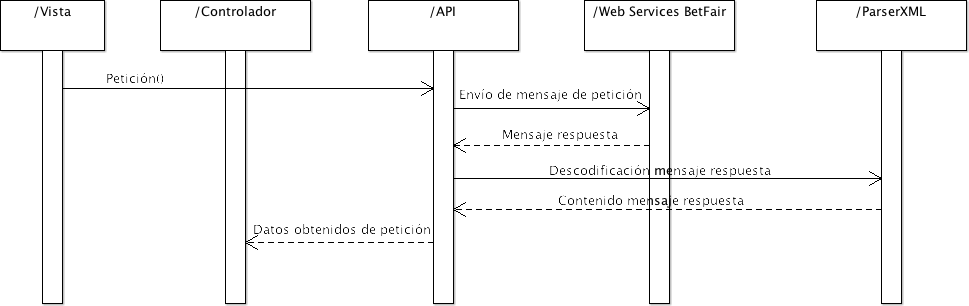
\includegraphics[width=1.2\textwidth]{./images/modelo_accion.png}
     \caption{Ejemplo de comunicación API }
   \label{fig:proceso}
\end{figure}
 
    
    Toda la aplicación gira en torno a este proceso. Sin él es incomprensible el resto del aplicativo. Es en él donde obtenemos los datos directamente de BetFair. Es lógico tratarlo así ya que las aplicaciones móviles suelen usar siempre servicios web y por tanto necesitan de conectividad. Esta aplicación no guarda información alguna salvo las credenciales de acceso al servicio. En una aplicación móvil nos interesa que la información que se necesita esté disponible cualquiera que sea el lugar donde nos encontremos. En el contexto de las apuestas lo más importante es tener la información lo más actualizada posible, es por eso que no se guarda la información de los mercados. Eso sí, tendría sentido quizá dotar en un futuro a la aplicación de una caché ,opcional a la elección del usuario, con caducidad para, por ejemplo, minimizar el consumo de batería del dispositivo en el caso que se necesitase.  
   
%%% Local Variables: 
%%% mode: latex
%%% TeX-master: "tfc-betfair-ios"
%%% TeX-PDF-mode: t
%%% ispell-local-dictionary: "castellano"
%%% End: 

\cleardoublepage
%%%%%%%%%%%%%%%%%%%%%%%%%%%%%%%%%%%%%%%%%%%%%%%%%%%%%%%%%%%%%%%%%%%%%%%%
\chapter{Conclusiones y Trabajo Futuro}
\label{ch:conclusiones}

\section{Conclusiones}
 El presente trabajo de Fin de Carrera consiste en el desarrollo de una herramienta software para manejar apuestas en Internet bajo los terminales móviles \emph{iOS}. 
 
Uno de los puntos claves del presente trabajo ha sido el portado de un servicio web originalmente diseñado para el mundo de navegadores web de PC a una plataforma móvil de última generación. En este trabajo de fin de carrera se ha elegido el \emph{API} de Betfair y podemos concluir que su portado ha sido exitoso. La clave de este éxito ha sido el diseño e implementación de un parser, explicado en el capítulo \ref{ch:implemetacion}, que hace de nexo de unión entre el servidor de Betfair y la aplicación. El parser realiza las funciones de un codificador y encapsulador de datos. En torno a él gira el resto del desarrollo.
 
 Se han implementado los servicios básicos del \emph{API}. Está limitación de servicios se ha debido al tipo de licencia elegido. Por este motivo se ha diseñado, desde el primer momento, una aplicación de tipo modular para que en un futuro se agreguen el resto de las funcionalidades sin ningún tipo de complicación. La arquitectura del desarrollo permite este tipo de ampliaciones siguiendo las técnicas de software específicas.
 
 Otro punto clave y diferenciador en este trabajo es la implementación de la funcionalidad de \emph{trading}, como vimos en el capítulo \ref{ch:intro}. La aplicación es capaz de recalcular las condiciones del mercado basándose en una apuesta ya realizada y asistir al usuario para una ganancia segura o minimizar la pérdida según la evolución del mercado. La arquitectura de la aplicación esta diseñada para que en un futuro cercano se pueda desarrollar esta funcionalidad para que se realice sobre múltiples eventos y mercados.
 
 Se ha conseguido no almacenar información localmente redundante de la aplicación. Debido al uso de servicios web todos los datos de consulta y de generación por parte del usuario se guardan en el servidor. Por lo tanto, si el usuario usa alguna otra aplicación en otra plataforma no sería necesario ningún mecanismo de sincronización de información. En este tipo de contextos es mejor disponer de datos lo más actualizados posibles directamente desde el servidor que manejar una caché de datos desactualizadas al poco tiempo de descargarse del servidor. Los mercados están en continua evolución.
 
 Otro objetivo cumplido es la implementación de la internacionalización de la aplicación. La aplicación estará disponible a través de la tienda \emph{iTunes} \emph{Store}. Esta tienda tiene un acceso mundial y debido a ello se ha adoptado los principales idiomas para que la aplicación sea lo más extendida posible. 
 
\section{Trabajo futuro}
 Como ya hemos visto en la arquitectura de la aplicación, el sistema está preparado para posibles futuras funcionalidades extras que podemos aportar con los datos que nos ofrece el API. Debido a que el núcleo de la aplicación es la obtención y proceso de la información contenida en Betfair, cualquier desarrollador puede añadir una funcionalidad extra usando los datos anteriores y acoplarlas fácilmente a la arquitectura de la aplicación. Al usar el modelo vista-controlador, la sencillez a la hora de implementar nuevas funcionalidades está mas que probada.
 
\subsection*{\emph{Trading} global por lista de eventos}
 Una mejora interesante a implementar en un futuro sería la de poder realizar \emph{trading} sobre un mercado entero. Al principio del presente trabajo hemos definido el \emph{trading} como apostar a favor y en contra de un evento determinado para, según nuestra primera apuesta, obtener beneficio seguro o minimizar la pérdida. Pero, apostar a favor de un evento ¿puede suponer que éste afecte al resto del mercado? Pongamos un ejemplo, supongamos que estamos apostando por quién va a ser el campeón del mundial de Sudáfrica. Apostar a favor de un equipo puede llevar la consecuencia de apostar en contra de los restantes participantes si en vez de pensar en un equipo concreto pensamos en el mercado completo. 
 
  Este cambio en nuestro planteamiento supone llevar a cabo un gran control sobre todas las variables que afectan al mercado completo y no sólo por un evento. Para poder analizar completamente los datos de mercado (cuota y precio) necesitamos analizar los datos concretos de cada evento de dicho mercado. Para poder obtener cual sería el conjunto de apuestas a realizar en el mercado para obtener el beneficio tenemos que resolver un conjunto de ecuaciones lineales que representan al mercado cuyas incógnitas serán las cuotas y cantidad a apostar por cada eventos de dicho mercado.    
  
 Normalmente los mercados tienen unos 30 eventos. Para poder obtener una solución óptima tenemos que echar mano de herramientas de software de resolución de ecuaciones lineales, tales como \emph{zympl} y \emph{glpsol}. 
  
  
  
   La idea es tener una máquina servidora capaz de realizar estos cálculos cada, pongamos por ejemplo, una hora. Se trata de analizar continuamente el mercado para encontrar el momento idóneo para el \emph{trading} global. El incluir otra máquina a parte del terminal es debido a la restricción de la batería. Si hiciéramos uso del terminal para estos cálculos reduciría drásticamente la vida útil de la misma. La máquina avisaría a la aplicación móvil del terminal en cuanto encontrase una solución adecuada a los parámetros configurados. 
   
    El procedimiento por el cual el usuario es notificado con la solución es implementar la solución de mensajería tipo \emph{push} de Apple en el \emph{iPhone}. A continuación mostramos como son las notificaciones en el terminal, también como mejora a añadir al proyecto.
    
 \subsubsection*{Notificación por mensajes \emph{Push} de Apple}
   
   En un modelo típico de cliente-servidor, el cliente es el encargado de contactar con el servidor para la descarga de nuevos datos, como por ejemplo el servicio de correo electrónico. En un dispositivo móvil, el cuál siempre tiene el inconveniente de la batería, esta solución no es válida debido al consumo energético en cada consulta al servidor. Para estos casos las notificaciones \emph{push} son las solución a este dilema. Una notificación \emph{push} es un mensaje corto que el servidor envía al cliente para notificarle que tiene datos para ser descargados o eventos pendientes tales como nueva versión de la aplicación. 
   
    Cuando un dispositivo móvil recibe una notificación de una aplicación que no está ejecutada en ese momento, el sistema notifica al usuario a través de un mensaje de alerta, un sonido determinado o un número indicador en el icono de la aplicación (o una combinación de este conjunto) de un evento a tratar por parte del usuario. El usuario, en todo momento, tiene la posibilidad de ejecutar la aplicación para obtener los datos notificados o simplemente ignorar el mensaje.

     \begin{figure}[h!]
    \centering
       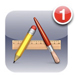
\includegraphics[width=0.2\textwidth]{./images/badged_app.jpg}
     \caption{Alerta 1 }
   \label{fig:Alerta 1}
\end{figure}

\begin{figure}[h!]
    \centering
       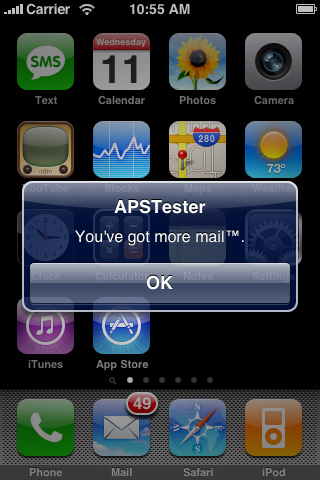
\includegraphics[width=0.3\textwidth]{./images/notif_msg_one_button.jpg}
     \caption{Alerta 2 }
   \label{fig:Alerta 2}
\end{figure}

\begin{figure}[h!]
    \centering
       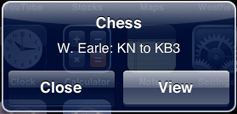
\includegraphics[width=0.3\textwidth]{./images/alert.jpg}
     \caption{Alerta 3 }
   \label{fig:Alerta 3}
\end{figure}

     
    Brevemente explicaremos el proceso completo del envío de un mensaje desde el servidor hasta la aplicación cliente del terminal. 
    
    En todo el proceso intervienen 3 actores: el servidor que desea entregar un mensaje, el servidor de Apple de envío de mensajes y la aplicación cliente.
    
 \begin{figure}[h!]
    \centering
       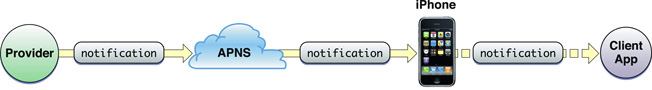
\includegraphics[width=0.95\linewidth]{./images/remote_notif_simple.jpg}
     \caption{Proceso general }
   \label{fig:Notificacion proceso}
\end{figure}

   \subsubsection*{Registro}

     El primer paso del proceso es el registro de la aplicación en el servidor de Apple para activar el servicio de notificaciones. Tal y como se muestra en la figura \ref{fig:Notificacion Registro}, la aplicación cliente se conecta al \emph{APNS}\footnote{Apple Push Notification Server, el servidor encargado de recibir y enviar el mensaje de un tercero a un terminal iphone} para la obtención de un identificador (\emph{token}) único para cada aplicación cliente y terminal. El APNS, después de comprobar las credenciales del terminal, genera y registra el \emph{token} a partir del ID del dispositivo y devuelve al terminal su \emph{token} generado. Este \emph{token} identifica al terminal y por lo tanto lo ha de usar nuestro servidor para poder enviar a este terminal un mensaje \emph{push}. Por eso, el último paso del registro es notificar al servidor desde el terminal el \emph{token} generado para su registro interno.
     
 \begin{figure}[h!]
    \centering
       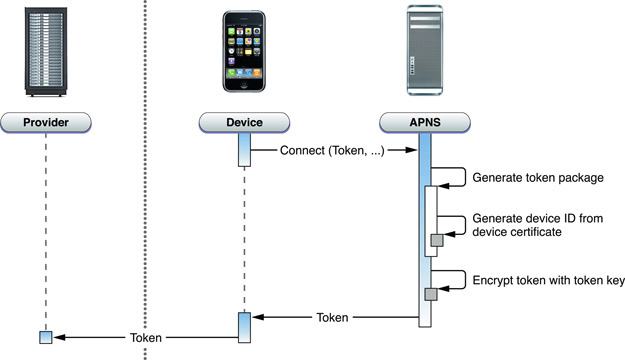
\includegraphics[width=0.8\textwidth]{./images/token_generation.jpg}
     \caption{Registro }
   \label{fig:Notificacion Registro}
\end{figure}
  
     \subsubsection*{Envío de una notificación}
     
     Tal y como se muestra en la figura \ref{fig:Notificacion envio} cuando el servidor requiere enviar una notificación a un cliente determinado para indicarle que dispone de datos nuevos que descargar, éste envía el mensaje en cuestión junto con el identificador del terminal al APNS. El servidor APNS comprueba que el \emph{token} ha sido generado por un certificado válido y que identifica a un terminal registrado previamente. Si todo esta correcto le envía el mensaje a la aplicación cliente del terminal.
     
 \begin{figure}[h!]
    \centering
       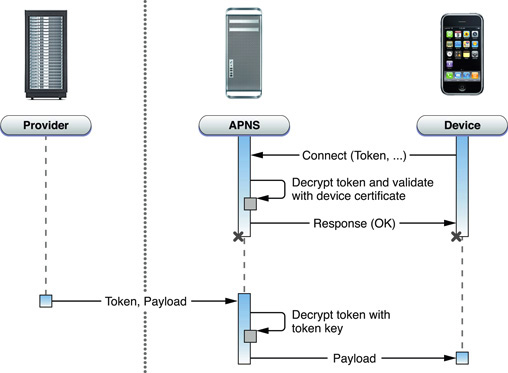
\includegraphics[width=0.8\textwidth]{./images/token_trust.jpg}
     \caption{Envío}
   \label{fig:Notificacion envio}
\end{figure}

 Como podemos ver, mediante estas notificaciones podemos tener al cliente lo más actualizado posible minimizando el gasto de batería si le tuviese que conectar periódicamente con algún servidor. \cite{betfair:web}

%%% Local Variables: 
%%% mode: latex
%%% TeX-master: "tfc-betfair-ios"
%%% TeX-PDF-mode: t
%%% ispell-local-dictionary: "castellano"
%%% End: 

\cleardoublepage

%%%%%%%%%%%%%%%%%%%%%%%%%%%%%%%%%%%%%%%%%%%%%%%%%%%%%%%%%%%%%%%%%%%%%%
%% COMIENZO DE LOS APÉNDICES
%% (NO TOCAR)
% \appendix

%%%%%%%%%%%%%%%%%%%%%%%%%%%%%%%%%%%%%%%%%%%%%%%%%%%%%%%%%%%%%%%%%%%%%%
%% APÉNDICES:
%%  * PONER CADA APÉNDICE EN UN FICHERO COMO SI FUERAN CAPÍTULOS
%%  * HACER UN include POR CADA FICHERO E INCLUIRLO EN includeonly
%%  * AÑADIR \clearemptydoublepage DESPUÉS DE CADA include
% \include{ej-apendice}
% \cleardoublepage

%%%%%%%%%%%%%%%%%%%%%%%%%%%%%%%%%%%%%%%%%%%%%%%%%%%%%%%%%%%%%%%%%%%%%%
%% COMIENZO DE LA BIBLIOGRAFÍA
%% (NO TOCAR)
\bibliographystyle{plain}
\addcontentsline{toc}{chapter}{Bibliografía}

%%%%%%%%%%%%%%%%%%%%%%%%%%%%%%%%%%%%%%%%%%%%%%%%%%%%%%%%%%%%%%%%%%%%%%
%% BIBLIOGRAFÍA
%% (AÑADIR FICHEROS .bib CON LA BIBLIOGRAFÍA USADA EN EL TFC)
\bibliography{betting}
\nocite{*}

\end{document}

%%% Local Variables: 
%%% mode: latex
%%% TeX-master: t
%%% TeX-PDF-mode: t
%%% ispell-local-dictionary: "castellano"
%%% End: 
